\documentclass[12pt]{article}
\usepackage{siunitx}
\usepackage{pgfplots}
\pgfplotsset{compat=1.18} % Or adjust depending on your TeX distribution
\usepackage[utf8]{inputenc}	% Para caracteres en español
\usepackage{amsmath,amsthm,amsfonts,amssymb,amscd}
\usepackage{multirow,booktabs}
\usepackage[table]{xcolor}
\usepackage{fullpage}
\usepackage{lastpage}
\usepackage{newtxmath}
\usepackage{newtxtext}
\usepackage{enumitem}
\usepackage{fancyhdr}
\usepackage{mathrsfs}
\usepackage{wrapfig}
\usepackage{setspace}
\usepackage{calc}
\usepackage{multicol}
\usepackage{cancel}
\usepackage[retainorgcmds]{IEEEtrantools}
\usepackage[margin=3cm]{geometry}
\usepackage{amsmath}
\newlength{\tabcont}
\setlength{\parindent}{0.0in}
\setlength{\parskip}{0.05in}
\usepackage{empheq}
\usepackage{framed}
\usepackage[most]{tcolorbox}
\usepackage{xcolor}
\colorlet{shadecolor}{orange!15}
\parindent 0in
\parskip 12pt
\geometry{margin=1in, headsep=0.25in}
\theoremstyle{definition}
\newtheorem{defn}{Definition}
\newtheorem{reg}{Rule}
\newtheorem{exer}{Exercise}
\newtheorem{note}{Note}
\newtheorem{theorem}{Theorem}
\setcounter{section}{0}
\usepackage{chngcntr}
\usepackage{hyperref}
\counterwithin*{equation}{section}
\counterwithin*{equation}{subsection}
\usetikzlibrary{angles,quotes,calc,positioning}
\usetikzlibrary{decorations.pathmorphing, patterns, calc}
\usepackage{mathtools} 
\begin{document}

\section{Info}

\begin{itemize}
    \item karinachattah@unc.edu.ar
\end{itemize}

\textbf{Temas:}

\begin{itemize}
    \item Cinemática y dinámica (mecánica)
    \item Campos eléctricos y magnéticos
    \item Circuitos 
    \item Termodinámica
\end{itemize}

\section{Measurements and magnitudes}

Measurements seek to compare a prediction with an observation, so as to test a
hypothesis. A magnitude is a number accompanied by a unit. Some magnitudes are: 

\begin{itemize}
    \item Length, measured in meters $(m)$
    \item Time, measured in seconds ($s$)
    \item  Mass, measusred in kilograms (kg)
    \item Current, measured in ampers ($A$)
    \item Temperature, measured in kelvins ($k$)
    \item Matter, measured in moles (mol)
\end{itemize}

We consider $10^3$ (e.g. kilometer) and $10^{-3}$ (e.g. milimiters) to be within
human scale.  We call mass, seconds and kilograms the \textit{mechanical units}.
We define the \textit{force unit}, or Newton, as

\begin{equation*}
    [F] = N = \text{kg} \frac{m}{s^2}
\end{equation*}

and the Pascal unit as 

\begin{equation*}
    [P] = \text{Pa} = \frac{N}{m^2}
\end{equation*}

We use scientific notation and terms which express quantities as powers of ten.
For instance, $10^{12}$ is the tera, $10^{3}$ the giga, etc.

The magnitudes hereby described are suited for algebraic manipulation. For
instance, $m \times m = m^2$, and $s \times \frac{m}{s} = m$.

\section{Vectors}

Vectors are used to express position, displacement, velocity, force,
acceleration, fields, etc. A vector $\overrightarrow{A}$ (or sometimes
$\overrightarrow{a}$) in the general sense has a direction (line), an
orientation, and a length (or magnitude). A vector also has an application
point, which denotes the point of origin of the vector. When saying $\overrightarrow{a}
= \overrightarrow{b}$, we mean that $\overrightarrow{a}$ and
$\overrightarrow{b}$ coincide in direction, magnitude and orientation,
irrespective of their application point. 

The scalar product is defined as the usual mapping in the space $\mathbb{R}^n
\times \mathbb{R} \mapsto \mathbb{R}^n$. Intuitively, the scalar product $\lambda
\overrightarrow{a}$
"streches" or "shrinks" a vector, depending on wheter $|\lambda| < 1$ or not,
and the positivty or negativity of $\lambda$ determines whether the vector
inverts its direction or not. In general, $\left| \lambda \overrightarrow{a}
\right| = \left| \lambda \right| \left| \overrightarrow{a} \right| $.

The sum of vectors, $\overrightarrow{a} + \overrightarrow{b}$, is a mapping
$\mathbb{R}^n \times \mathbb{R}^n \mapsto \mathbb{R}^n$. As usual, and in a
graphical sense, the sum corresponds to the application of the parallelogram
rule. 

\begin{shaded}
    \textbf{Parallelogram rule}. Make $\overrightarrow{a}$ and
    $\overrightarrow{b}$ coincide in their point of application. From the tip of 
    $\overrightarrow{a}$, draw a copy of $\overrightarrow{b}$, and from the tip
    of $\overrightarrow{b}$ a copy of $\overrightarrow{a}$. The corner of the
    thus generated parallelogram is the tip of $\overrightarrow{a} +
    \overrightarrow{b}$.

    Alternatively, from the tip of $\overrightarrow{a}$ write
    $\overrightarrow{b}$. Then $\overrightarrow{a} + \overrightarrow{b}$ is the
    vector which goes from the point of application of $\overrightarrow{a}$ to
    the tip of $\overrightarrow{b}$.
\end{shaded}

The sum of vectors is commutative, associative, and distributive with respect to
scalar product.

If $\overrightarrow{A}$ is a vector, we use $A_x$ and $A_y$ to denote the
projection of the vector over the axis $x$ or $y$, respectively. Using $A_x$ and
$A_y$ one forms a rectangular triangle with sides $A_x$, $A_y$ and a hypotenuse 
of length $\left| \overrightarrow{A} \right| $. 

Let $\theta$ be the angle formed
by $\overrightarrow{A}$ with the $x$-axis. Then, using trigonometry,

\begin{equation*}
    \cos \theta = \frac{A_x}{\left| \overrightarrow{A} \right| }, \qquad \sin
    \theta = \frac{A_y}{\left| \overrightarrow{A} \right| }
\end{equation*}

from which one can find $A_x, A_y$ assuming one knows $\theta$. From this
follows that $\left| \overrightarrow{A} \right| $ and $\theta$ fully determine
all the information about the vector, insofar as the allow us to determine $A_x,
A_y$. Conversely, knowing $A_x$ and $A_y$ is also sufficient to determine
$\overrightarrow{A}$, insofar as 

\begin{equation*}
    \left| \overrightarrow{A} \right|  = \sqrt{A_x^2 + A_y^2} , \qquad \frac{A_y}{A_x} =
    \frac{\left| \overrightarrow{A} \right| \sin \theta}{\left|
    \overrightarrow{A} \right|  \cos \theta} = \tan \theta \Rightarrow \theta =
    \arctan \left( \frac{A_y}{A_x} \right) 
\end{equation*}

As convention, we use $\hat{i}$ to denote the versor (vector of length 1) with
direction parallel to the $x$-axis, and $\hat{j}$ the versor with direction
parallel to the $y$-axis.

Notice that, for any vector $\overrightarrow{A}$, $A_x$ is $\hat{i}$ times
$A_x$, and $A_y$ is $\hat{j}$ times $A_y$, which means 

\begin{equation*}
    \overrightarrow{A} = A_x \hat{i} + A_y \hat{j}
\end{equation*}

When writing $\overrightarrow{A}$ in this way, we say we write it in term of its
components $x, y$. In terms of linear algebra, it's not hard to see that we are
simply expressing that $\hat{i}, \hat{j}$  form a basis of $\mathbb{R}^2$. Thus,
it is equivalent to write 

\begin{equation*}
    A_x = \left| \overrightarrow{A} \right|  \cos \theta, \qquad A_y = \left|
    \overrightarrow{A} \right| \sin \theta
\end{equation*}

and 

\begin{equation*}
    \overrightarrow{A} = \left| \overrightarrow{A} \right| \left( \cos \theta
    ~ \hat{i} + \sin \theta ~ \hat{j}\right) 
\end{equation*}

From this follows as well that 

\begin{align*}
    \overrightarrow{A} + \overrightarrow{B} 
    &= \left( A_x \hat{i} + A_y \hat{j} \right) + (B_x \hat{i} + B_y \hat{j}) \\ 
    &= \hat{i}\left( A_x + B_x \right)  + \hat{j}\left( A_y + B_y \right) 
\end{align*}

which means the sum of vectors has as components the sum of the components.

The scalar product of two vectors, $\overrightarrow{A} \cdot
\overrightarrow{B}$, is a scalar defined as 

\begin{equation*}
    \overrightarrow{A} \cdot \overrightarrow{B} = \left| \overrightarrow{A} \right| \left| \overrightarrow{B} \right| \cos \theta
\end{equation*}

where $\theta$ is the angle formed by the two vectors. The scalar product is
positive if $\cos \theta$ is positive, which occurs for $0 < \theta \leq 90$. It
is negative if $\cos \theta $ is negative, i.e. if $90 < \theta \leq 180$.
Clearly, $\overrightarrow{A} \cdot \overrightarrow{B} = 0 \iff \theta = 90$.

In general, from the definition follows that

\begin{equation*}
    \overrightarrow{A} \cdot \overrightarrow{B} = A_x B_x + A_y B_y
\end{equation*}

The vectorial product $\overrightarrow{A} \times \overrightarrow{B}$ is a vector
perpendicular to the plane formed by $\overrightarrow{A}$ and
$\overrightarrow{B}$. Its module is $\left| \overrightarrow{A} \right| \left|
\overrightarrow{B} \right| \sin \theta $, and its direction is given by what's
called the right-hand rule.

\pagebreak 

\subsection{Excercises}

\begin{shaded}
    \textbf{(2)} Sean los vectores $\overrightarrow{A} = 2\hat{i} + 3\hat{j}$
    $\overrightarrow{B} = 4\hat{i} -2 \hat{j}$ y $\overrightarrow{C} = -\hat{i}
    + \hat{j}$.
    Determinar la magnitud y el ángulo (representación polar) de los vectores
    resultantes $\overrightarrow{D} = \overrightarrow{A} + \overrightarrow{B} +
    \overrightarrow{C}$ y $\overrightarrow{E} = \overrightarrow{A} +
    \overrightarrow{B} - \overrightarrow{C}$. Resolver analítica y
    gráficamente.
\end{shaded}

(Analytical solution.) We'll use $A_x, A_y$ to denote the components of the
vector $\overrightarrow{A}$, and same for all other vectors. We know the
components of $\overrightarrow{D}$ are 

\begin{equation*}
    D_x = A_x + B_x + C_x = 2 + 4 - 1 = 5, \qquad D_y = 3 - 2 + 1 = 2
\end{equation*}

from which readily follows that $\left| D \right| = \sqrt{5^2 + 2^2} = \sqrt{29}
\approx 5.385$. Similarly, 

\begin{equation*}
    E_x = 2 + 4 + 1 = 7, \qquad E_y = 3 - 2 -1 = 0
\end{equation*}

from which follows that $\left| E \right| = \sqrt{7^2} = 7 $.

Now, we must recall that 

\begin{equation*}
    \theta_{\overrightarrow{Z}} = \arctan \left( \frac{Z_y}{Z_x} \right) 
\end{equation*}

for any $\overrightarrow{Z}$.


We need not memorize this: it is trigonometrically clear that 
$Z_x = \cos \theta_{\overrightarrow{Z}} \left| \overrightarrow{Z} \right| $ and 
$Z_y = \sin \theta_{\overrightarrow{Z}} \left| \overrightarrow{Z} \right| $, and
therefore 

\begin{equation*}
    \frac{Z_y}{Z_x} = \tan \theta
\end{equation*}

And $\arctan$ is the inverse of $\tan$. Anyhow, for $\overrightarrow{E}$ and
$\overrightarrow{D}$ we have 

\begin{equation*}
    \theta_{\overrightarrow{E}} = \arctan\left( \frac{E_y}{E_x} \right) =
    \arctan\left( 0 \right) = 0
\end{equation*}

\begin{equation*}
    \theta_{\overrightarrow{D}} = \arctan\left( \frac{D_y}{D_x} \right) =
    \arctan \left( \frac{2}{5} \right) \approx 0.38
\end{equation*}

\pagebreak 

\begin{shaded}
    \textbf{(3)} Can two vectors of different magnitud be combined and yield zero? What about three?
\end{shaded}

The zero vector is the only vector with magnitude zero. Let $\overrightarrow{A},
\overrightarrow{B}$ arbitrary vectors. Then 

\begin{equation*}
    \left| \overrightarrow{A} + \overrightarrow{B} \right| = \sqrt{(A_x + B_x)^2
    + (A_y + B_y)^2} 
\end{equation*}

which is zero if and only if 

\begin{equation*}
    ( A_x + B_x )^2 + ( A_y + B_y )^2 = 0
\end{equation*}

This only holds if $A_x + B_x = A_y + B_y = 0$. But 

\begin{equation*}
    A_x + B_x = 0 \Rightarrow A_x = -B_x, \qquad A_y + B_y = 0 \Rightarrow A_y =
    -B_y
\end{equation*}

But then 

\begin{equation*}
    \left| A \right| = \sqrt{A_x^2 + A_y^2} = \sqrt{(-B_x)^2 + (-B_y)^2} =
    \sqrt{B_x^2 + B_y^2}  = \left| B \right| 
\end{equation*} 

$\therefore ~ \left| \overrightarrow{A} + \overrightarrow{B} \right| = 0 \iff
\left| \overrightarrow{A} \right| = \left| \overrightarrow{B} \right| $.

It is simple to see that three vectors of different magnitude can add to zero.

\pagebreak 

\begin{shaded}
    Assume $A + B + C = 2\hat{i} + \hat{j}$ and $A = 6\hat{i}-3\hat{j}, B =
    2\hat{i} + 5\hat{j}$. Find the components of $C$. Solve analytically and
    graphically.
\end{shaded}

We know 

\begin{equation*}
    6 + 2 + C_x = 2, \qquad -3 + 5 + C_y = 1
\end{equation*}

from which follows that $C_x = -6, C_y = -1$.

\pagebreak 

\begin{shaded}
    \textbf{(5)} $A$ and $B$ have a magnitud of $3m, 4m$ respectively. The angle between them
    is $\theta = 30$ degrees. Find their scalar product.
\end{shaded}

Their scalar product is 

\begin{equation*}
    ( \left| B \right|  \cos \theta ) \left| A \right| 
\end{equation*}

Recall that 

\begin{equation*}
    \text{Angle in degrees} = \text{Angle in radians} \cdot \frac{180}{\pi}
\end{equation*}

Thus, thirty degrees equates to $30 \frac{\pi}{180} \approx 0.523$ radians. Then
the scalar product is 

\begin{equation*}
    4 \cos (0.523) \times 3 \approx 10.395
\end{equation*}




\pagebreak 

\begin{shaded}
    \textbf{(6)} Find the angle between $A = 4 \hat{i} + 3 \hat{j}$ and 
    $B = 6\hat{i} - 3 \hat{j}$.
\end{shaded}

Recall that 

\begin{equation*}
    A \cdot B = \left| A \right| \left| B \right| \cos \theta
\end{equation*}

where $\theta$ is the angle between the vectors. This readily entails that 

\begin{equation*}
    \frac{A \cdot B}{\left| A \right|\left| B \right|  } = \cos \theta
\end{equation*}

or equivalently that 

\begin{equation*}
    \theta = \arccos \left( \frac{A \cdot B}{\left| A \right|\left| B \right|  } \right)  
\end{equation*}

Now, $A \cdot B = 4 \times 6 + 3 \times -3 = 24 - 9 = 15$ and $\left| A \right|
\left| B \right| = 5 \cdot 6.708 = 33.541 $.

Therefore, 

\begin{equation*}
    \theta = \arccos \left( \frac{15}{33.541} \right) = \arccos \left( 0.447
    \right) = 1.107
\end{equation*}

\pagebreak 

\begin{shaded}
    \textbf{(7)} Let $\overrightarrow{v} = \left( \frac{1}{3}, \frac{2}{3} \right) $ be the vector of
    components. Find the components of the vector of module 5 whose direction 
    and orientation (sentido) are those of the given vector.
\end{shaded}

Assume $\overrightarrow{x} = (x_1, x_2)$ is of magnitude $5$. Any vector whose
direction and orientation are the same than those of $\vec{v}$ is "a stretching"
of $\vec{v}$. In other words, for $\vec{x}$ to satisfy the requirements, we must
have 

\begin{equation}
    \vec{x} = \lambda \vec{y}
\end{equation}

for some $\lambda \in \mathbb{R}$. (Furthermore, $\lambda > 0$ since otherwise
orientation is not preserved.) 

Now, from equation $(1)$ follows that

\begin{equation}
    \|\vec{x}\| =  \lambda \|\vec{y}\|
\end{equation}

since the magnitude of a scaled vector is the scaled magnitude of the vector.
Equation $(2)$ simplifies to 

\begin{equation}
    \|\vec{x}\|  = \lambda \sqrt{1 / 9 + 4 / 9} = \frac{\lambda
    \sqrt{5} }{3}
\end{equation}

From this readily follows that $\frac{3}{\sqrt{5} }\|\vec{x}\| = \lambda$. But
it is a hypothesis that $\|\vec{x}\| = 5$. Therefore, 

\begin{equation}
    \lambda = \frac{3}{\sqrt{5} } \cdot 5 = \frac{15}{\sqrt{5} }
\end{equation}

In other words, 

\begin{equation}
    \vec{x} = \frac{15}{\sqrt{5} } \vec{v} 
\end{equation}

which is ugly but can be simplified.


\pagebreak 

\begin{shaded}
    \textbf{(8)} Write the expression of the vector product $\vec{c} = \vec{u}
    \times \vec{v}$ in the following cases: 

    \begin{enumerate}
        \item $\vec{u}, \vec{v}$ are coplanar. Provide a graphical
            interpretation. 
        \item $\vec{u} = 2\hat{i} - 3 \hat{j} + \hat{k}$ and $\vec{v} =
            -3\hat{i} + \hat{j} + 2 \hat{k}$. Find the module of the resulting
            vector $\vec{c}$ in two different ways.
    \end{enumerate}
\end{shaded}

$(1)$ Two vectors are coplanar if there is a plane which contains them both.
Since the vector product $\vec{u} \times \vec{v}$ is a vector orthogonal 
to both $\vec{u}$ and $\vec{v}$


\pagebreak 

\begin{shaded}
    \textbf{(12)} Un avión vuela 200 km hacia el NE en una dirección que forma
    un ángulo de 30 hacia el este de la dirección norte. En ese punto cambia su
    dirección de vuelo hacia el NO. En esta dirección vuela 60 km formando un
    ángulo de 45 con la direccióon norte.

    (a) Calcular la máxima distancia hacia el este del punto de partida a la que
    llegó el avión. 

(b) Calcular la máxima distancia hacia el norte del punto de partida a la que
llegó el avión. 

(c) Calcular la distancia a la que se encuentra el avión del punto de partida al
cabo de su recorrido. 

(d) Determinar vectorialmente el camino que debería hacer para volver al punto
de partida. Resolver gráfica y analíticamente.
\end{shaded}

Sea $\vec{A}$ el vector que describe el primer recorrido, $\vec{B}$ el
vector que describe el segundo recorrido. Al final del problema, el avión se
encuentra en la posición indicada por $\vec{A} + \vec{B}$. 

Como $\vec{A}$ describe un movimiento con un ángulo de $\theta = 60$ grados
($90 - 30$) respecto al eje $y$ (norte), y una magnitud de 200km, podemos
determinarlo recordando que

\begin{equation*}
     A_x = \left| \vec{A} \right| \cos \theta, \qquad A_y = \left| \vec{A}
     \right| \sin \theta
\end{equation*}

En radianes, $\theta = \frac{\pi}{180} \times 60 = 1.047$

\begin{equation*}
    A_x = 200 \times \cos \left( 1.047 \right) = 100.034, \qquad A_y = 22 \times
    \sin(1.047) = 173.185
\end{equation*}

En conclusión, $\vec{A} = 100.034 \hat{i} + 173.185 \hat{j}$. Mismo razonamiento
nos da que el ángulo del segundo vector es de $130$ grados, lo cual en radianes
nos da $\alpha = \pi / 180 \times 130 = 2.268$. Por ende, 

\begin{equation*}
    B_x = 60 \cos(2.268) = -38.524, \qquad B_y = 60  \sin(2.268) = 45.998
\end{equation*}

Es decir que $\vec{B} = -38.524 \hat{i} + 45.998 \hat{j}$. De esto se sigue 
que $\vec{C} = \vec{A} + \vec{B} = (61.51, 219.183)$. 

$(a)$ Claramente, es la coordenada $x$ del vector $\vec{A}$, $100.034$.

$(b)$ Claramente, es la coordenada $y$ del vector $\vec{C}$: $218.183$. 

$(c)$ Claramente, es la magnitud de $\vec{C}$, es decir $\|\vec{C}\| =
\sqrt{61.51^2 + 219.183^2} = 227.65$.

$(d)$ El camino para volver es dado por $\vec{C} \times (-1)$.

















\pagebreak

\section{Cynematics}


\subsection{Unidimensional movement}

The study of movement requires two variables: position ($x$, in units of length)
and time ($t$, in seconds). We begin our study with unidimensional movement,
i.e. movement which occurs along a single axis. 

Experimentally, a way to study unidimensional movement could consist in taking a
sequence of photographs (from the same position and angle) of the moving object
at times $t_1, \ldots, t_n$. Some coordinate system must be imposed upon the
space along which the object moves, e.g. setting an axis with origin at the
initial position of the object, the same direction as the movement of the
object, and some appropriate units. The photographs would then provide a
sequence of positions $x_1, \ldots, x_n$.

Clearly, $\left\{ t_n \right\}, \left\{ x_n \right\}  $ could be understood as
defining a discrete function $\varphi(n)$, which on its turn might be
interpolated to obtain a continuous approximation $\phi(t)$. To the limit, the
continuous approximation converges to what we call a movement function. 

\begin{shaded}
    \textbf{Movement function}. A movement function $x(t)$ is a continuous,
    smooth function.

    \textbf{Examples.} $x(t) = c$ (reposo), $x(t) = at + b$ (MRU), $x(t) = at^2
    + bt  + c$ (MRUV).
\end{shaded}

\subsection{Coincidence, displacement, temporal intervals}

If $A, B$ are objects with movement functions $x_A(t), x_B(t)$, we say $A, B$
coincide (se encuentran) when $x_A(t) = x_B(t)$.

We define displacement (desplazamiento) (relative to positions $x_1, x_2$) as
$\Delta x = x_2 - x_1$. Notice that $\Delta x$ is not the same as distance: if
one travels from $A$ to $B$ and then to $B$ from $A$, the distance traveled is
to times the distance from $A$ to $B$, but $\Delta x = 0$.

We also define a temporal interval, relative to two times $t_1, t_2$, as $\Delta
t = t_2 - t_1$, where $t_2 > t_1$. 

\subsection{Velocity}

We define \textit{median velocity} (velocidad media) as 

\begin{equation}
    \overline{v} = \frac{\Delta x}{\Delta t} = \frac{x_2 - x_1}{t_2 - t_1}
\end{equation}

where $x_2 = x(t_2), x_1 = x(t_1)$. Clearly, $\overline{v}$ is the slope of the
line which intersects $x(t)$ at points $t_1, t_2$. The sign of $\overline{v}$
then determines the direction (sentido) of movement. The unit of $\overline{v}$
is then $L / T$ (length over time), for instance kilometers per hour. Median
velocity indicates the rate of change of distance in time.

Clearly, an object in reposo has a median velocity of zero. An object with
movement function $x(t) = at + b$ (MRU) has median velocity $a$. The case of
interest is an object with a quadratic movement function (MRUV).

If $x(t) = at^2 + b t + c$, let $m$ the midpoint of the quadratic expression and 
take $t_1 = m - c, t_2 = m + c$ with $c > 0$. Clearly, the median velocity from 
$t_1$ to $m$ is negative, that from $m$ to $t_1$ is positive, and that from 
$t_1$ to $t_2$ is zero. This is sufficient to suggest that median velocity does
not clearly express the nature of the movement. 

For that reason, the length $\Delta$ of the interval $[t_1, t_2]$ might be
reduced in the limit to zero, so that we get an accurate notion of the
instantaneous (or close to instantaneous) change of direction. Needless to say,
the limit converges to the slope of the line  tangent to $(t_1, x(t_1))$, i.e.
the derivative of $x(t)$ at $t_1$. Thus, we obtain the definition of
instantaneous velocity, usually called simply velocity: 

\begin{equation}
    v(t) = \lim_{\Delta t \to 0} \frac{\Delta x}{\Delta t} = \frac{dx}{dt} =
    v'(t)
\end{equation}

Again, $\left[ v(t) \right] = \frac{L}{T}$. Quite clearly, $v(t) = \overline{v}$
for constant and linear functions, but for the quadratic function $x(t)$ we
have 

\begin{equation*}
    x(t) = at^2 + b t + c, \qquad v(t) = 2at + b
\end{equation*}





\pagebreak
\section{De adelante hacia atrás}

Recordemos que si $x(t)$ es función de movimiento, $v(t) = \frac{dx}{dt}$ es la
velocidad, y $a(t) = \frac{d^2 x}{dt^2}$ es la aceleración. Naturalmente, esto
significa que 

\begin{equation*}
    x(t) = \int v(t') dt' + D, \qquad v(t) = \int a(t') dt' + C
\end{equation*}

donde $D, C$ son constantes de movimiento que dependerán de las condiciones
iniciales.

\begin{shaded}

\textbf{$( \dagger )$ Derivada y puntos de inflexión}
Un punto de inflexión de $f$ continua y dos veces derivable en $[a, b]$ es un
valor $x_0 \in [a, b]$ t.q. $f^{(2)}(x_0) = 0$. Los puntos de inflexión
representan un cambio de comportamiento en $f$, en particular transiciones de
cóncava a convexa y viceversa.

Intuitivamente, y  exceptuando casos límite (como $f''$ constante), si $f''(x_0) = 0$, entonces alrededor de $x_0$ hay un cambio de
signo en $f''$, lo cual quiere decir que en el entorno alrededor de $x_0$ la
función original pasa de crecer a decrecer, o de decrecer a crecer.

\end{shaded}

\pagebreak 

\section{Movimiento bidimensional (cinemática 2D)}

Se modela con una curva en el plano cartesiano. La curva (el dibujo del
movimiento) se denomina trayectoria. La trayectoria \textit{no} es una función,
obviamente (e.g. una circunferencia es una trayectoria posible).

La descripción de la posición del objeto en cada instante de tiempo $t$ se
descsribe con vectores. En el plano cartesiano, decimos que $\vec{r} = \hat{x}i
+ y \hat{j}$
es un vector posición si la punta de $\vec{r}$ se corresponde con la posición
del objeto (en un tiempo dado).

Sea $\theta$ el ángulo formado por $\vec{r}$ y el eje $x$, de manera tal que $x
= \left| \vec{r} \right| \cos \theta, y = \left| \vec{r} \right| \sin \theta$.
Es decir, $\vec{r} = \left| \vec{r} \right| \cos \theta \hat{i} + \left|
\vec{r}\right| \sin \theta \hat{j} $.

Ahora pensemos el objeto en movimiento, y que registramos a lo largo del tiempo
$t$ las posiciones $x(t), y(t)$. Claramente, $x(t), y(t)$ son funciones de
movimiento unidimensionales. Por lo tanto, podemos definir el vector posición de
manera general como 

\begin{equation}
    \vec{r}(t) = x(t)\hat{i} + y(t) \hat{j}
\end{equation}

Ahroa consideremos la trayectoria $T$ (conjunto de puntos en el eje cartesiano)
del objeto. Sean $P_1, P_2 \in T$ dos puntos en el plano que pertenecen a la
trayectoria. Definimos el desplazamiento del objeto como 

\begin{equation}
    \Delta \vec{r} = \vec{r_2} \vec{r_1}
\end{equation}

donde $\vec{r_1}, \vec{r_2}$ son los vectores con puntas en $P_1, P_2$. De esto
se sigue que 


\begin{equation}
    \Delta \vec{r} = \vec{r}(t_2) - \vec{r}(t_1)
\end{equation}


para dos instantes de tiempo $t_1, t_2$. Además, es claro que $\Delta\vec{r}$ es
el vector que conecta las dos puntas, desde $P_1$ hasta $P_2$, y que $\vec{r_2}
= \vec{r_1} + \Delta \vec{r}$. 

La velocidad media en el intervalo de tiempo $[t_1, t_2]$ se define entonces
como 

\begin{equation}
    \overline{v}_{[t_1, t_2]} = \frac{\Delta \vec{r}}{\Delta t} = 
    \frac{\vec{r}(t_2)-  \vec{r}(t_1)}{t_2 - t_1}
\end{equation}

lo cual es claramente un vector que contendrá las velocidades medias en las
direcciones $x$ e $y$. El vector velocidad entonces se define como uno
esperaría: 

\begin{align}
    \vec{v}(t) 
    &= \lim_{\Delta t \to 0}  \frac{\Delta \vec{r}}{\Delta t}  \\
    &= \lim_{\Delta t \to 0} \frac{\vec{r}(t_2)-  \vec{r}(t_1)}{t_2 - t_1}
    \nonumber \\
    &= \frac{d \vec{r}}{dt} \nonumber \\ 
    &= \frac{d}{dx} \left( x(t)\hat{i} + y(t) \hat{j} \right) \nonumber\\ 
    &= \frac{dx}{dt} \hat{i} + \frac{dy}{dt} \hat{j} \nonumber
\end{align}

Por lo tanto, 

\begin{equation}
    \vec{v}(t) = v_x(t) \hat{i} + v_y(t) \hat{j}
\end{equation}

con $v_x, v_y$ las velocidades correspondientes a las funciones de movimiento $x(t), y(t)$.

\begin{shaded}

    $(\dagger)  \textbf{ Interpretación gráfica de $\vec{v}$}$. Gráficamente, el
    vector velocidad $\vec{v}(t)$ se representa como sigue. Imagine la
    trayectoria $T$ y un vector posición $\vec{r}$ que conecta con $P \in T$.
    Entonces $\vec{t}$ será paralelo a la recta tangente a la trayectoria $T$ en
    el punto $P$. Esto \textit{no} es una derivada, porque la trayectoria $T$ no
    es una función. En otras palabras, el vector velocidad es tangente a la
    trayectoria.
\end{shaded}

Definimos entonces el versor 

\begin{equation}
    \hat{v} = \frac{\vec{v}}{\left| \vec{v} \right| }
\end{equation}

que nos da la dirección tangencial de la velocidad. 

Así como tenemos un vector velocidad, tenemos el vector aceleración 

\begin{equation}
    \vec{a}(t) = \frac{d^2 x}{dt^2} \hat{i} + \frac{d^2 y}{dt^2} \hat{j}
\end{equation}

de acuerdo al mismo razonamiento límite que nos dio el resultado $(6)$. El
vector aceleración también puede descomponerse en sus direcciones tangencial y
normal (respecto a la trayectoria). La aceleración tangencial será la dirección
de la velocidad: 

\begin{equation}
    \text{aceleración tangencial} \to  \hat{v} = \frac{\hat{v}}{\left| \vec{v}
    \right| }, \qquad \text{aceleración normal} \to \hat{n} = (\bot  \vec{v})
\end{equation}

donde $\bot \hat{v}$ es el vector tal que $\bot  \hat{v} \cdot \hat{v} = 0$
(perpendicular). 

\begin{shaded}
    $(\dagger)$ \textbf{ Algunas observaciones}. Hablemos en un intervalo de
    tiempo $[t, t + \Delta t]$.

    $(a)$ Cuando $\vec{v}$ cambia de módulo y de sentido, pero no de dirección,
    la aceleración es puramente tangencial, es decir está en la dirección de la
    velocidad. (Son paralelos.) 

    $(b)$ Cuando $\vec{v}$ cambia de dirección y de sentido, pero no de módulo
    (i.e. el vector apunta hacia otro lado pero tiene el mismo largo), se cumple
    que la aceleración es perpendicular a la velocidad. Es decir, es puramente
    normal.

    $(c)$ Si $\vec{v}$ cambia de módulo, de sentido y de dirección, el vector 
    $\vec{a}$ tendrá una componente tangencial y normal.

    La aceleración puramente  tangencial resulta en un movimiento
    unidimensional, una línea recta. El caso $(b)$ corresponde a un movimiento
    bidimensional.
\end{shaded}

\subsection{Tiro de proyectil}

El tiro de proyectil es un movimiento bidimensional bajo la acción única de la
gravedad. Si imaginamos la parábola de un proyectil, surgen preguntas cómo cuál
es su altura máxima, su destino final, etc. Asumamos que se ha impuesto un
sistema de coordenadas.

Observemos que el objeto \textit{no} tiene aceleración en el eje $x$, sólo
velocidad. En el eje $y$ el proyectil es afectado por la gravedad.
Por ende, 

\begin{equation*}
\vec{a} = o \hat{i} - 9.8 \frac{m}{s^2} \hat{j}
\end{equation*}

Luego, en $t = 0$, 

\begin{align*}
    \vec{v_0} = v_{0x} \hat{ i} + v_{0y} \hat{j} = \vec{v}(t = 0)
\end{align*}

Asumamos que por convención, $\vec{r}(t = 0) = 0$. Por ende, 

\begin{equation*}
    \vec{r}(t = 0) = x_0 \hat{i} + y_0 \hat{j} 
\end{equation*}

Entonces, 

\begin{align*}
    \vec{v}(t) = v_{0x} \hat{i} - ( 9.8 \frac{m}{s^2}t + v_{0y} ) \hat{j}
\end{align*}

Integrando una vez más, 

\begin{equation*}
    \vec{r}(t) 
    = ( v_{0x}t + x_0 ) \hat{i} + \left( - 9.8 \frac{m}{s^2}
    \frac{t^2}{2} + v_{0y}t + y_0 \right)  \hat{j}\\ 
\end{equation*}

Pero $\vec{r}(t) = x(t) \hat{i} + y(t) \hat{j}$. Por ende, 

\begin{equation*}
    x(t) = v_{0x} t + x_0, \qquad y(t) = - 9.8 \frac{m}{s^2} \frac{t^2}{2} +
    v_{0y}t + y_0
\end{equation*}

Vemos entonces que $x(t)$ es lineal, y su pendiente es la velocidad inicial (en
$x$) dada por $v_{0x}$. $y(t)$, por otro lado, es cuadrática con máximo. Dicho
máximo se corresponde con el punto más alto. Es decir, el punto más alto ocurre
en el tiempo $t_m$ tal que

\begin{equation*}
    v_y(t_m) = 0 \implies t_m = \frac{v_{0y}}{9.8 \frac{m}{s^2}}
\end{equation*}

El tiempo de vuelo está dado por el tiempo en que la altura se hace cero, es
decir el $t_{\text{vuelo}}$ tal que $y(t_{\text{vuelo}}) = 0$. Es la raíz máxima
de
$y(t)$. La trayectoria será despejando $t$ de $x$: 

\begin{equation*}
    t = \frac{x - x_0}{v_{0x}}
\end{equation*}

La trayectoria también será una parábola, en este caso particular. Y como en
cada punto la aceleración es la aceleración negativa de la gravedad, los
vectores aceleración a lo largo del tiempo serán siempre "flechas rectas hacia
abajo".

\pagebreak
\section{Descripción vectorial del movimiento}

Usamos $\vec{r}(t)$ para denotar al vector posición, $\vec{v}(t)$ para denotar
al vector velocidad, y $\vec{a}(t)$ para denotar al vector aceleración. Si
$x(t), y(t)$ son las funciones de movimiento en los ejes $x, y$, entonces 

\begin{equation}
    \vec{r}(t) = x(t) \hat{i} + y(t) \hat{j}, \qquad \vec{v}(t) = \frac{dx}{dt}
    \hat{i} + \frac{dy}{dt} \hat{j}, \qquad \vec{a}(t) = \frac{d^2 x}{dt^2}
    \hat{i} + \frac{d^2 y}{dt^2} \hat{j}
\end{equation}

y \begin{equation}
    \left| \vec{r} \right| = \sqrt{x^2 + y^2}
\end{equation}

Dados dos instantes $t_1 < t_2$, el desplazamiento del un objeto en movimiento
con vector posición $\vec{r}(t)$ es el vector 

\begin{equation*}
    \Delta\vec{r} := \vec{r}(t_2) - \vec{r}(t_1)
\end{equation*}

Notar que este es el vector que "parte" de la punta de $\vec{r}(t_1)$ y llega a
la punta de $\vec{r}(t_2)$. Es decir, marca desde dónde y hasta dónde se movió
el cuerpo en el tiempo $[t_1, t_2]$.

La velocidad media del cuerpo en el intervalo $[t_1, t_2]$ es el vector
velocidad media: 

\begin{equation*}
    \overline{\vec{v}(t_1, t_2)} := \frac{\Delta \vec{r}}{\Delta t} = \frac{\vec{r}(t_2) -
\vec{r}(t_1)}{t_2 - t_1}
\end{equation*}

o equivalentemente 

\begin{equation}
    \overline{\vec{v}(t, \Delta t)} := \frac{\vec{r}(t + \Delta t) - \vec{r}(t)}{\Delta t}
\end{equation}

Puesto que $\overline{\vec{v}}$ se obitene multiplicando $\Delta \vec{r} =
\vec{r}(t_2) - \vec{r}(t_1)$ por un escalar positivo, ambos vectores tendrán
misma dirección y sentido.  Es decir, la velocidad media es paralela y
equidireccional al desplazamiento.

Respecto al vector velocidad, en un punto dado de la trayectoria, no es difícil
ver que "ocupa" un segmento de la recta tangente a la trayectoria en dicho
punto. 

With regards to the acceleration vector, we note that 

\begin{equation*}
    \vec{a} = \vec{a}_t + \vec{a}_n
\end{equation*}

where $\vec{a}_t$ is the \textit{tangential acceleration} and $\vec{a}_n$ the
normal acceleration. The tangential acceleration operates along the directoin of
the velocity, affecting the speed of the object. Normal acceleration is
perpendicular to velocity, and it afects the direction of the object. Objects
moving in a straight line have a null normal acceleration, since their direction
doesn't change. Objects moving in curvilinear fashion always have non-null
normal acceleration (and hence non-null acceleration). 

If the velocity is constant, such as in uniform circular motion, $\vec{a}_t = 0$
and therefore $\vec{a}$ is purely orthogonal to the velocity. If velocity is
not constant but changing, then $\vec{a}$ has a component along the velocity and
it is not perpendicular to it.

\pagebreak

\section{Dinámica Newtoniana}

There in this world are four fundamental forces: gravitational, electromagnetic,
strong nuclear, and weak nuclear. The first two are the ones we experience in
our daily lives. The strong and weak nuclear forces operate at the atomic level,
and are not relevant to our discussion. 

The gravitational force is an attractive force which operates between any two
masses. The electromagnetic force operates between any two charged particles,
and can be attractive or repulsive. We will discuss now the gravitational force.

Formally, we define $\vec{F} = F_x \hat{i} + F_y \hat{j} + F_z \hat{k}$ to be a
force. The unit of force is the Newton ($N$), which is defined as the force
required to accelerate a mass of $1 kg$ at a rate of $1 m/s^2$.  

Newton discovered fundamental laws of motion, which we summarize here: 

\begin{shaded}
    \textbf{Newton's First Law (Law of Inertia).} An object at rest remains at
    rest, and an object in motion continues in motion with constant velocity,
    unless acted upon by a net external force. 

    \begin{equation}
        \vec{F}_T = 0 \Rightarrow \vec{v} = \text{constant}
    \end{equation}

    \textbf{Newton's Second Law.} The net force acting on an object is equal to
    the time rate of change of its momentum. If the mass of the object is
    constant, this is equivalent to saying that the net force acting on an
    object is equal to the product of its mass and its acceleration:

    \begin{equation}
        \vec{F}_{\text{T}} = m \vec{a}
    \end{equation}

    \textbf{Newton's Third Law.} If object $A$ exerts a force $\vec{F}$ on
    object $B$, then $B$ exerts a force $-\vec{F}$ on $A$. In other words,
    forces always come in pairs, equal in magnitude and opposite in direction.
    
\end{shaded}

We know 

\begin{equation*}
    \vec{v} = \int \vec{a}(t) ~ dt + \vec{C}, \qquad \vec{r} = \int \vec{v}(t) ~
    dt
\end{equation*}

Now, note that 

\begin{equation*}
    \vec{F}_T = F_{Tx}\hat{i} + F_{Ty} \hat{j}
\end{equation*}

and since $\vec{F}_T = m \vec{a}$

\begin{equation*}
    \vec{a} = \frac{ \vec{F}_T }{m} =  \frac{F_{Tx}\hat{i} + F_{Ty} \hat{j}}{m}
    = a_x \hat{i} + a_y \hat{j}
\end{equation*}

Then 

\begin{equation}
    \vec{a} =  \frac{ \vec{F} }{m} = \frac{d^2 \vec{r}}{dt^2}
\end{equation}

Furthermore, 

\subsection{Tipos de fuerzas}

There are many types of forces, but we will discuss only a few. The MRU
(movimiento rectilíneo uniforme) is a movement with no forces acting on the
object. The MRUV (movimiento rectilíneo uniformemente variado) is a movement
with a constant force acting on the object. 

\begin{equation*}
    \sum \vec{F} = 0 \Rightarrow \vec{v} = \text{constant}, \vec{a} = 0 \qquad \text{(MRU)}
\end{equation*}

\begin{equation*}
    \vec{F} = \text{constant} \Rightarrow \vec{a} = \text{constant} = \vec{F}/m
\end{equation*}

The gravitatory force is an example of a constant force producing MRUV. 

Another force is denote by tension (tensión). It is the force exerted by a rope,
string, cable, etc. It is always directed along the rope, and it can be
attractive or repulsive. The cable is assumed to be massless and inextensible.
It transmits the same force throughout its length.

Another force is the contact force (fuerza de contacto). It is the force exerted
by a surface on an object in contact with it. It is always perpendicular to the
surface. It is sometimes called the normal force. It is a rule that 

\begin{equation*}
    \vec{a} = 0 \implies \vec{N} + \vec{P} = 0
\end{equation*}

Another force is the elastic force (fuerza elástica). It is the force
exerted by a spring when it is stretched or compressed. It is given by Hooke's
law: 

\begin{equation*}
    \vec{F}_e = - k \Delta \vec{x} = -k (x - \ell_0)\hat{i}
\end{equation*}

where $k$ is the spring constant, and $\Delta \vec{x}$ is the displacement
vector of the spring from its equilibrium position. The negative sign indicates
that the force exerted by the spring is in the opposite direction to the
displacement. 

Another force is the centripetal force (fuerza centrípeta). It is the force
that keeps an object moving in a circular path. It is always directed towards
the center of the circle. 

Another force is the gravitational force (fuerza gravitatoria). 
It is the force exerted between two masses without contact. It is given by
Newton's law of universal gravitation: 

\begin{equation*}
    \vec{F}_g = - G \frac{m_1 m_2}{r^2} \hat{r}
\end{equation*}

where $G$ is the gravitational constant, $m_1, m_2$ are the masses of the two
objects, $r$ is the distance between them, and $\hat{r}$ is the unit vector
pointing from one mass to the other. The negative sign indicates that the force
is attractive. The force exerted by both objects is equal in magnitude and
opposite in direction, in accordance with Newton's third law.












\pagebreak


\subsection{Excercises}

\begin{shaded}
    \textbf{(1)} Consider 

    \begin{equation*}
        x(t) = 1 \left[ \frac{m}{s^2} \right] t^2 - 3 \left[ \frac{m}{s} \right]
        t
    \end{equation*}

    the movement function of a body travelling in a straight line, with $x$ 
    in meters and $t$ in seconds. 

    $(a)$ Plot $x(t)$

    $(b)$ Determine analytically the median velocity in $[-1, 5], [-1, 8], [-1,
    0.9], [-1, 0.99], [ -1, 0.999]$.

    $(c)$ Let $\Delta t_n = t_n - t_0$ with $\left\{ t_n \right\} = \left\{ -1,
    5, 4, 1, -0.5, -0.8, -0.9, - 0.99, -0.999\right\}  $ all measured in
    seconds. To what value does the median velocity of the object converge as
    $t_n$ decreases in the interval $[-1, -1 + \Delta t_n]$? What is the
    geometrical interpretation of this
    result? 

    $(d)$ Find the equation for the line tangent to $x(t)$ at $t = -1 s$.
\end{shaded}

$(a)$ Notice that since $t$ is in seconds, $\frac{mt^2}{s^2}$ correctly
expresses a quantity in meters, and so does $\frac{mt}{s}$. So we will from now
on write simply $x(t) = t^2 - 3t$, understanding that it is a mapping from time
in seconds to meters.

\begin{tikzpicture}
  \begin{axis}[
      axis lines = middle,
      xlabel = {$t$ (s)},
      ylabel = {$x(t) = t^2 - 3t$},
      domain=-2:2,   % time range
      samples=100,
      grid=both,
      thick
    ]
    % Plot x(t) = t^2 - 3t
    \addplot[blue, thick] {x^2 - 3*x};
    \node[above right] at (axis cs:3,0) ;
  \end{axis}
\end{tikzpicture}


$(b)$ The median velocity of an object in the time interval $[t_a, t_b]$  was
given by 

\begin{equation}
    \frac{\Delta x}{\Delta t} = \frac{ x(t_b) - x(t_a) }{t_b - t_a}
\end{equation}

So excercise $(b)$ is as simple as plugging in the corresponding values into
equation $(1)$ and I skip  it. 

$(c)$ Let $t$ be an arbitrary value. Then by definition of $\frac{dx}{dt}$,

\begin{equation*}
    \lim_{\Delta t \to 0 } \frac{x(t + \Delta t) - x(t)}{(t + \Delta t) -
    t} =\lim_{\Delta t \to 0 } \frac{ x(t + \Delta t) - x(t) }{\Delta t} = \frac{dx}{dt}
\end{equation*}

the derivative of $x(t)$ at time $t$. In particular, the limit whose convergence
we are asked to study is nothing but the limit above with $t = -1$:

\begin{equation*}
    \lim_{\Delta t \to 0 } \frac{x(-1 + \Delta t) - x(-1)}{\Delta t} = x'(-1)
\end{equation*}

So suffices to observe that $x'(t) = 2t - 3$ and $x'(-1) = -5$. In conclusion, 
the object at time $t = -1$ travels at an instantaneous velocity of $-5$ meters
per second.

$(d)$ The line $\ell(t) = at + b$ tangent to $x(t)$ at $t = -1s$ has slope $a =
-5$ and crosses through the point $(-1, 4)$. So we must have $-5(-1) + b = 4
\iff b = 4 - 5 = -1$. So the line is $\ell(t) = -5t - 1$.

\pagebreak 

\begin{shaded}
    \textbf{(4)} Answer the questions.
\end{shaded}

$(a)$ Can an object have null velocity and yet possess acceleration?  


\small
\begin{quote}

Let $x(t)$ the describe the movement of the object and $v(t) = x'(t)$ its
velocity, both as a function of time. Assume for an arbitrary $t_0$ that 
$v(t) = 0$. It is very much possible that $v'(t_0) \neq 0$.  

Consider, for instance, that $v(t)$ is linear and non-constant, making $v'(t) =
a$ a non-null constant. Then there exists a unique root $r$ s.t. $v(r) = 0$, but
independently of this fact $v'(r) = a \neq 0$.

Physically, it should be clear that if a non-moving object could not possess
acceleration, then it would be impossible for it to pass from a still to a
moving state. So, at least at the intutition level, this \textit{reductio ad
absurdum} suffices.

\end{quote}
\normalsize

$(b)$ Can a moving object have a null displacement in a given interval and yet
non-null velocity?


\small
\begin{quote}

Naturally. Take as example an object moving in circles at a constant, non-null
velocity $v$, and assume it travels a full circle in $t$ seconds. Then all of
the intervals in $\left\{ [t_0, t_0 + tk] : k \in \mathbb{N} \right\} $ are such
that they give null displacements. Yet the object \textit{is} moving.

\end{quote}
\normalsize

$(c)$ Can an object have an east-bound velocity of while its acceleration is
west-bound?


\small
\begin{quote}

Informally, this is quite clearly the case, insofar as any positively-moving
object whose velocity decreases must have a negative acceleration.

\end{quote}
\normalsize

$(d)$ Consider an object moving on a straight line, with the east being the positive
direction, under a velocity of $v(t) = 20 \text{ms}^{-1} - 2 \text{ms}^{-2} t$.
For $t = 0\text{s}, t = 1\text{s}$, what is the situation?


\small
\begin{quote}

Its velocity is clearly positive in both cases (20 and 18), evidently
decreasing, which points out the fact that its acceleration is negative (-2).

\end{quote}
\normalsize

$(e)$ A ball is thrown vertically. What do the \textit{signs} of velocity and
acceleration look like as the object ascends, and what does that mean? And
when the object descends? What happens at the highest point?


\small
\begin{quote}

Clearly, its velocity is positive during the ascending phase, and negative
during the descending phase. At the highest point, the velocity will be exactly
zero. 

Conversely, acceleration is always negative due to the force excercised by
gravity on the ball. 

It is the fact that acceleration is constantly negative what causes the ball not
only to lose velocity as it goes up until it begins to fall again, but to then
fall more and more rapidly as time goes by.


\end{quote}
\normalsize

\pagebreak 

\begin{shaded}
    \textbf{(5)} A particle moves through the $x$-axis with movement function 
    $x(t) = 3 + 17t - 5t^2$, with $x$ in meters and $t$ in seconds. 

    $(a)$ What is the position of the particle at times $\left\{ 1, 2, 3
    \right\} $?

    $(b)$ At what point in time does the particle return to the origin? 

    $(c)$ Find $v(t)$ and determine the instantaneous velocity at times $\left\{
    1, 2, 3\right\} $. When is the velocity null? What is the particles velocity
    when it crosses the origin? 

    $(d)$ Plot $x(t), v(t), a(t)$.
\end{shaded}


$(a)$ Trivial, simply compute $x(1), x(2), x(3)$.

$(b)$ See that

\begin{equation*}
    x(t) = 0 \iff t = \frac{17}{10} \pm \frac{ \sqrt{17^2 + 4\times 3 \times 5}
    }{10}
\end{equation*}

which gives approximate solutions $t_1 \approx -0.168, t_2 \approx 3.568$. It
makes no sense to speak of negative time and we keep only the positive solution
$t = 3.568$. Thus, the particle returns to the origin after approximately 3.568
seconds.

$(c)$ The first derivative of $x(t)$ is 

\begin{equation*}
    v(t) = -10t + 17
\end{equation*}

The instantaneous velocity at times 1, 2, 3 are $v(1) = 7, v(2) = -3, v(3) = -13$.

\begin{equation*}
    17 = 10t \iff t = \frac{17}{10} = 1.7
\end{equation*}

The particle crosses the origin at approximately time $3.568$ and its velocity
is approximately $v(3.568) = -18.682$. 

$(d)$ The acceleration is constant: $a(t) = -10$.

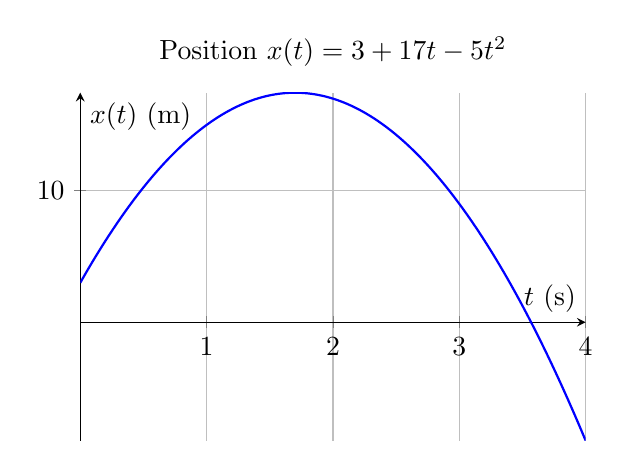
\begin{tikzpicture}
\begin{axis}[
    width=8cm,
    height=6cm,
    axis lines=middle,
    xlabel={$t$ (s)},
    ylabel={$x(t)$ (m)},
    domain=0:4,
    samples=200,
    grid=both,
    title={Position $x(t)=3+17t-5t^2$}
]
\addplot[blue, thick] {3 + 17*x - 5*x^2};
\end{axis}
\end{tikzpicture}

\vspace{1cm}

% --- Velocity v(t) ---
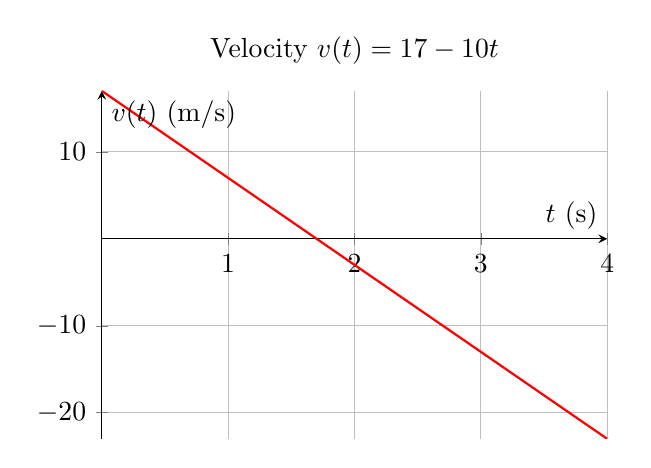
\begin{tikzpicture}
\begin{axis}[
    width=8cm,
    height=6cm,
    axis lines=middle,
    xlabel={$t$ (s)},
    ylabel={$v(t)$ (m/s)},
    domain=0:4,
    samples=200,
    grid=both,
    title={Velocity $v(t)=17-10t$}
]
\addplot[red, thick] {17 - 10*x};
\end{axis}
\end{tikzpicture}

\vspace{1cm}

% --- Acceleration a(t) ---
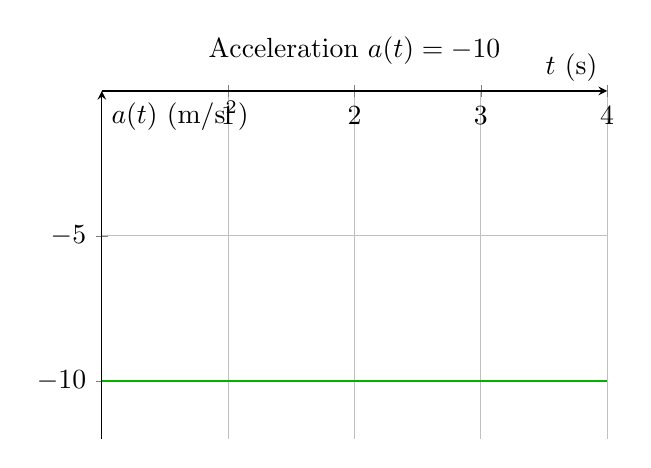
\begin{tikzpicture}
\begin{axis}[
    width=8cm,
    height=6cm,
    axis lines=middle,
    xlabel={$t$ (s)},
    ylabel={$a(t)$ (m/s$^2$)},
    domain=0:4,
    samples=2,
    grid=both,
    title={Acceleration $a(t)=-10$},
    ymin=-12, ymax=0
]
\addplot[green!70!black, thick] {-10};
\end{axis}
\end{tikzpicture}

\pagebreak 

\begin{shaded}
    (\textbf{6}) $(a)$ Determine the instantaneous acceleration of the object
    plotted in the exercise for $t = 3, t = 11$.

    $(b)$ Compute the distanace traveled by the object in the time intervals
    $[0, 5]$ and $[0, 9]$ and $[0, 15]$.

    $(c)$ Knowing that $x(t = 6) = 0$, find the position of the object at $t =
    0$. 

    $(d)$ Give an expression for the objects position for all $t$. 

    $(e)$ Plot $x(t), v(t), a(t)$.
\end{shaded}

The velocity of the object is constantly $20$m/s from time $t = 0$ to time $t =
6$. Then it linearly increases until it reaches $44$m/s at $t=9$, from whereon
it linearly decreases until it reaches $0$ms at time $t = 15$.

The linear expression $\ell_1(t) = a_1t + b_1$ which satisfies $\ell(6)=20,
\ell(9) = 44$ is such that 

\begin{equation*}
    6a_1 + b_1 = 20, \qquad 9a_1 + b_1 = 44
\end{equation*}

The associated system of equations yields that $b_1 = 20 - 6a_1$, from which
follows that $9a_1 + (20 - 6a_1) = 44$, entailing 

\begin{equation*}
    a_1 = \frac{24}{3} = 8
\end{equation*}

From this readily follows that $b_1 = 20 - 6\times 8 = -28$. 

Similarly, the linear expression $\ell_2(t) = a_2t + b_2$ which gives a line
s.t. $\ell_2(9) = 44, \ell_2(15) = 0$ must satisfy 

\begin{equation*}
    9a_2 + b_2 = 44, \qquad 15a_2 + b_2 = 0
\end{equation*}

Then $b_2 = -15a_2$ and $9a_2 -15a_2 = 44$, entailing $a_2 = -\frac{22}{3}$.
From this follows that $b_2 = 110$ via simple calculations. Thus, 


\begin{equation*}
    v(t) = \begin{cases}
        20 & 0 \leq t \leq 6 \\ 
        8t - 28 & 6 < t \leq 9 \\ 
        -\frac{22}{3}t + 110 & 9 < t \leq 15
    \end{cases}
\end{equation*}

It should be intuitive to graps that the distance travelled $d(a, b)$ in the interval
$[a, b]$ is

\begin{equation*}
    d(a, b) = \int_a^b |v(t)| ~ dt
\end{equation*}

If $v(t)$ is in meters per second, and $t$ is in seconds, the total number of
meters travelled in a time interval $[a, b]$ is the summation of the meters per
second travelled in every instant! This will involve the anti-derivative of 
$v(t)$, i.e. the movement function $x(t)$, which we might as well compute at
once. 

\begin{align*}
    x(t) 
    &= \int v(t) ~ dt \\ 
    &= \begin{cases}
        20t + C_1 & 0 \leq t \leq 6 \\ 
        8\frac{t^2}{2} - 28t + C_2 & 6 < t \leq 9 \\ 
        -\frac{22}{3} \frac{t^2}{2} + 110t + C_3 & 9 < t \leq 15
    \end{cases} \\ 
    &= \begin{cases}
        20t + C_1 & 0 \leq t \leq 6 \\ 
        4t^2 - 28t + C_2  & 6 < t \leq 9 \\ 
        -\frac{22}{6} t^2 + 110t + C_3& 9 < t \leq 15
    \end{cases}
\end{align*}

The constants $C_1, C_2, C_3$ must satisfy the restriction of continuity and of
preserving the necessary values. In particular, we need $20(0) + C_1 = 20$.
Since we know $x(6) = 0$, we need $120 + C_1 = 0$, i.e. $C_1 = -120$. We also
need 

\begin{equation*}
    4(6^2) - 28(6) + C_2 = 0
\end{equation*}

to ensure continuity, so

\begin{equation*}
    C_2 = 24
\end{equation*}

Then we can know what $x(9)$ is and deduce $C_3$, which ends up being $-597$.

\begin{equation*}
    \therefore ~ x(t) = \begin{cases}
        20t - 120 & 0 \leq t \leq 6 \\ 
        4t^2 -28t + 24 & 6 < t \leq 9 \\ 
        -\frac{22}{6}t^2 +100t - 597 & 9 < t \leq 15
    \end{cases}
\end{equation*}

In any case, we could have computed the distance travelled without $x(t)$ (I
computed $x(t)$ because it's part of the exercise):

\begin{align*}
    d(0,5) 
    &= \int_0^5 v(t) ~ dt  \\ 
    &= 20 \times t]_0^5 \\ 
    &= 20 \times (5) \\ 
    &= 100
\end{align*}

\begin{align*}
    d(0, 9) 
    &= \int_0^6 v(t) ~ dt + \int_6^9 v(t) ~ dt \\ 
    &= 20 \times t\Big]_0^6 + (4t^2 - 28t)\Big]_6^9 \\ 
    &=120 + \left[ (4 \times 81 - 28 \times 9) - (4 \times 38 - 28 \times 6)
    \right]  \\ 
    &= 120 + 96 \\ 
    &= 216
\end{align*}

etc.

\pagebreak 

\begin{shaded}
    \textbf{(7)} A car and a truck leave at the same instant, the car initially
    being a certain distance behind the truck. The latter has a constant
    acceleration of $1.2 m / s^2$, while the car accelerates at $1.8 m / s^2$. 
    The car reaches the truck when the latter has covered 45 meters. 

    $(a)$ How much time does it take for the car to reach the truck?

    $(b)$ What is the initial distance between both vehicles?

    $(c)$ What is the velocity of each in the moment the cross paths? 

    $(d)$ Plot $x(t), v(t), a(t)$.
\end{shaded}

$(a)$ Since both vehicles have constant accelerations, they have linear
velocities and therefore quadratic movement functions. They will meet 
when the parabolas corresponding to these functions intersect. 

Let $x_1(t)$ denote the movement function of the car, $x_2(t)$ that of the
truck. We then wish to find the solutions to $x_1(t) = x_2(t)$. Now, 


\begin{equation}
    v_1(t) = \int a_1(t) = \int 1.8 ~ dt = 1.8 t + C_1
\end{equation}

\begin{equation}
    v_2(t) = \int a_2(t) = \int 1.2 ~ dt = 1.2 t + C_2
\end{equation}


are the velocities of the car ($v_1$) and the truck $(v_2)$. Since at $t = 0$
the velocities of both vehicles is zero (they start from rest), it is necessary
that $C_1 = C_2 = 0$. 

We know that the car reaches the truck when the latter has covered 45 meters, so
the question is what is the time $t_0$ when the distance covered by the truck is
that one? In other words, we need to find $t_0$ such that 

\begin{align*}
&\int_0^{t_0} v_2(t) ~ dt = 45 \\ 
    \iff&\int_0^{t_0} 1.2t ~ dt = 45 \\ 
    \iff&\left[ 0.6t^2  \right]_0^{t_0} = 45 \\ 
    \iff&0.6 t_0^2  =45 \\ 
    \iff & t_0 = \sqrt{75}  = \sqrt{25 \times 3}  = 5\sqrt{3} 
\end{align*}

Thus, the vehicles meet at time $t_0 = 5\sqrt{3}  $.

$(b)$ The initial distance between both vehicles is given by $\left| x_1(0) -
x_2(0) \right| $. From the velocities $v_1, v_2$ we can determine that 

\begin{equation}
    x_1(t) = 0.9t^2 + C_1', \qquad x_2(t) = 0.6t^2 + C_2'
\end{equation}

Let us fix our coordinate system so that the starting position of the truck
corresponds to the origin. Then $C_2' = 0$. Knowing that both vehicles coincide
at time $t_0 = 5\sqrt{3} $, we also know $X_1(t_0) = x_2(t_0)$, i.e.

\begin{equation}
    0.9(25 \times 3) + C_1' = 0.6(25 \times 3) 
\end{equation}

which entails $67.5 + C_1' = 45$, from which follows  that $C_1' = -22.5$. Thus,
the original distance of both vehicles is $22.5$m.

$(c)$ This consists simply of computing $v_1(t_0), v_2(t_0)$. Trivial.

$(d)$ Meh. 

\pagebreak 

\begin{shaded}
    \textbf{(8)} A car travels parallel to a train rail. The car stops at a red
    light in the exact instant when a train passes with a constant velocity of
    12m/s. The car remains at halt for 6s and then continues with a constant
    acceleration of $2m / s^2$.

    $(a)$ Determine the time it takes for the car to reach the train, with $t =
    0$ being the instant in which the car halted. 

    $(b)$ Determine the distance traveled by the car from the red light until it
    reached the train. 

    $(c)$ Determine the car's velocity at the instant it reaches the train.
\end{shaded}

$(a)$ Let $a_1(t)$ be the acceleration of the car, defined as 

\begin{equation}
    a_1(t) = \begin{cases}
        0 & 0 \leq t < 6 \\ 
        2 & t \geq 6
    \end{cases}
\end{equation}

Let $v_2(t) = 12 m / s$ be the constant velocity of the train. Let the point of
halt be the origin of our coordinate system, so that at time $t = 0$ (when the
car halted) both the train and the car are at position zero. Observe then that
it follows that $x_2(t) = 12t$ (in meters) via integration of $v_2(t)$ and the
necessary condition of the constant of integration being zero.

Integration of equation $(6)$ gives

\begin{equation}
    v_1(t) = \begin{cases}
        C_1 & 0 \leq t < 6 \\ 
        2t + C_2 & t \geq 6
    \end{cases} 
\end{equation}

where the constants of integration must satisfy two constraints: $(a)$ $v_1(0) =
0$ and $v_1$ must be continuous. From this follows that $C_1 = 0$ and that 
$2(6) + C_2 = 0$, i.e. $C_2 = -12 $. Therefore, 

\begin{equation}
    v_1(t) = \begin{cases}
        0 & 0 \leq t < 6 \\ 
        2 t - 12 & t \geq 6
    \end{cases}
\end{equation}

Via integration of $v_1$,

\begin{equation}
    x_1(t) = \begin{cases}
        C_1' & 0 \leq t < 6 \\ 
        t^2 -12 t + C_2' & t \geq 6
    \end{cases}
\end{equation}

Again, $C_1'$ must of course be zero, and $x_1(6)$ must also be zero, meaning
that $C_2 = -36 + 12(6) = 36$. Therefore,

\begin{equation}
    x_1(t) = \begin{cases}
        0 & 0 \leq t < 6 \\ 
        t^2 -12 t + 36 & t \geq 6
    \end{cases}
\end{equation}

The car reaches the train at the time $t_0 > 6$ which satisfies $x_1(t_0) =
x_2(t_0)$, so we solve

\begin{equation*}
    t^2 - 12t + 36 = 12t \iff t^2 - 24t + 36 = 0
\end{equation*}

which has solutions

\begin{equation*}
    \frac{24}{2} \pm \frac{\sqrt{24^2 - 4 \times 36} }{2} = 12 \pm 
    \frac{\sqrt{432} }{2} \approx 12 \pm 10.392
\end{equation*}

Keeping only the positive solution, we have that $t_0 \approx 22.392$. 


$(b)$ The distance traveled by the car from the red light until it reached the
train is the distance traveled from $t = 0$ to $t = t_0$, i.e. 

\begin{equation*}
    \int_0^{t_0} v_1(t) ~ dt = |x_1(t_0) - x_1(t_0)| = x_1(t_0) \approx 268.697
\end{equation*}

where the equality above holds only because velocity is always positive (i.e.
the car moves only in one direction).

$(c)$ Simply computing $v_1(t_0)$ gives the answer.

\pagebreak 

\begin{shaded}
    \textbf{(9)} A ball is thrown vertically and upwards from the floor with
    initial velocity $v_0$. Write the equations for the movement of the ball and
    plot graphically the vectors $\vec{y}(t), \vec{v}(t), \vec{a}(t)$. Identify
    the conditions for the instant of maximum height and the instant it reaches
    the floor.
\end{shaded}

The move is strictly vertical, so $\vec{r}(t) = 0\hat{i} + y(t)\hat{j}$ and we
need only determine the unidimensional vertical movement function $y(t)$.
Now, the ball is affected only by gravitiy, i.e. it is subjected to a constant
acceleration of $\vec{a}(t) = 0\hat{i} -9.8 \frac{m}{s^2}\hat{j}$. From this we
can derive the vertical velocity: 

\begin{equation*}
    v_y(t) = -9.8 \int ~ dt = -9.8t + C
\end{equation*}

The constant of integration must satisfy the initial velocity being $v_0$, so we
must have  

\begin{equation*}
    v_y(t) = v_0 - 9.8t
\end{equation*}

From this follows that 

\begin{equation*}
    r_y(t) = \int v_0 - 9.8t ~ dt = v_0t - \frac{9.8}{2}t^2 + C'
\end{equation*}

If we assume the position on the floor (vertically) is zero, we must have 
$C' = 0$, and 

\begin{equation*}
    r_y(t) = v_0t - 4.9t^2
\end{equation*}

In summary, 

\begin{equation*}
    \vec{r}(t) = 0\hat{i} - (v_0t - 4.9t^2)\hat{j}, \qquad \vec{v}(t) = 0\hat{i}
    - 9.8t \hat{j}, \qquad \vec{a}(t) = 0 \hat{i} - 9.8 \hat{j}
\end{equation*}

Maximum hight will occur at time $t \neq 0$ when the vertical velocity of the
ball is exactly zero. So, we solve 

\begin{equation*}
    v_0 - 9.8t = 0 \iff \frac{v_0}{9.8} =t
\end{equation*}

It will reach the floor at time $t \neq 0$ when the vertical position of the
ball is zero, so we solve 

\begin{equation*}
    v_0 t - 4.9t^2 = 0 \iff t(v_0 - 4.9t) = 0
\end{equation*}

The root $t = 0$ is not a solution that interests us, so we only care about the
root that solves $v_0 - 4.9t = 0$, i.e. $t = \frac{v_0}{4.9}$.

\pagebreak 

\begin{shaded}
    \textbf{(10)} A rock is thrown vertically and upwards. On its path, it
    crosses point $A$ with velocity $v$ and point $B$, which is $3$m higher than
    $A$, at velocity $v / 2$. Determine $v$ an the maximum height reached by the
    rock above point $B$.
\end{shaded}

Let $\Delta y = y_B - y_A = 3$m the distance between $A$ and $B$. We know the
rock has a constant acceleration $-g$ due to gravity. This tells us that
velocity is linear and movement is quadratic. In  general, 

\begin{equation*}
    a(t) = -g, \qquad v(t) = v_0 - gt, \qquad x(t) = y_0 + v_0 t - g\frac{t^2}{2}
\end{equation*}

Now, given an arbitrary velocity $v$ occurring when the object is at position
$y$,

\begin{equation*}
    \frac{dy}{dt} = v, \qquad \frac{dv}{dt} = a
\end{equation*}

assuming a constant acceleration $a$. However, since the position $y$ is a
function of time, the chain rule gives

\begin{equation*}
    \frac{dv}{dt} = \frac{dv}{dy} \frac{dy}{dt} = \frac{dv}{dy} v
\end{equation*}

From this follows $a = v \frac{dv}{dy}$ or equivalently $a ~ dy = v ~ dv$.
Integrating from initial positions and velocities $y_0, v_0$;

\begin{align*}
    &\int_{y_0}^y a ~ dy = \int_{v_0}^v v ~ dv 
    \\\Rightarrow ~ ~  &v^2 - v_0^2 = 2a(y -
    y_0)
\end{align*}

In other words, for any given velocity $v$ occurring at position $y$, the
relationship above holds. In particular, if we treat $A$ as our initial
position,

\begin{equation*}
    \frac{v^2}{4} - v^2 = 2a(y_B - y_A)
\end{equation*}

Since $y_B - y_A = 3$m,


\begin{equation*}
    \frac{v^2}{4} - v^2 = 6a
\end{equation*}

Now, the acceleration in our problem is simply $-g$, and then the equation above
gives solutions for $v$ given by

\begin{align*}
    &\frac{-3v^2}{4} = -6g \\ 
    \iff &v^2 = 8g \\ 
    \iff&v = \pm\sqrt{8g} 
\end{align*}

Now, since velocities can only be positive, we keep $v = \sqrt{8g} $ as the only
solution.

Now the question is, what is the maximum height? Well, in the path from $B$ to
the top, velocity drops from $\frac{v}{2}$ to zero. So again, if we take as
reference $B$, 

\begin{equation*}
    0 - \left( \frac{v}{2} \right) ^2 = 2a(y_{\text{top}} - y_B)
\end{equation*}

Let $h = y_{\text{top}} - y_B$. Then 

\begin{equation*}
    h = -\frac{v^2}{8a}
\end{equation*}

But $a = -g$ and $v = \sqrt{8g} $, giving 

\begin{equation*}
    h = \frac{8g}{8g} = 1
\end{equation*}

So the maximum height above $B$ is 1 meter.

\pagebreak 

\begin{shaded}
    \textbf{(11)} The movement in the plane of a particle is given by $x(t) =
    at^2$, $y(t) = b t ^3$, with $a = 3\frac{m}{s^2}, b = 2\frac{m}{s^3}$.

    $(a)$ Find the trajectory of the particle. Plot it. 

    $(b)$ Compute the acceleration at $t = 12$s. 

    $(c)$ What is the angle formed by the velocity vectors and the acceleration
    at that instant? 

    $(d)$ Determine the instant $t_1$ where acceleration is parallel to the line
    $y = x$, and the instant $t_2$ in which velocity is parallel to said line. 

    $(e)$ Determine the median velocity in the interval $(t_1, t_2)$.
\end{shaded}

$(a)$ 
The trajectory of the particle is 

\begin{align*}
    S 
&= \left\{ (x(t), y(t)) : t \in
\mathbb{R} \right\}  \\ 
&= \left\{ (3t^2, 2t^3) : t \in \mathbb{R} \right\} 
\end{align*}

Since $x = 3t^2, t^2 = \frac{x}{3}$. And since $y = 2t^3$, we have 
$y^2 = 4t^6 = 4 (t^2)^3 = 4\left( \frac{x}{3} \right)^3 = \frac{4}{27}x^3 $. In
summary, 

\begin{equation*}
    y^2 = \frac{4}{27}x^3
\end{equation*}

or equivalently 

\begin{equation*}
    y = \pm \frac{2}{3}\sqrt{x^3} 
\end{equation*}

This entirely defines $S$.


\begin{tikzpicture}[scale=0.05]
  \draw[->] (-5,0) -- (220,0) node[right] {$x$};
  \draw[->] (0,-200) -- (0,200) node[above] {$y$};

  % upper branch
  \draw[domain=0:200,smooth,variable=\x,red,thick]
    plot ({\x},{ sqrt(4/27*\x*\x*\x) });
  % lower branch
  \draw[domain=0:200,smooth,variable=\x,red,thick]
    plot ({\x},{ -sqrt(4/27*\x*\x*\x) });
\end{tikzpicture}


$(b)$ Clearly, 

\begin{equation*}
    v_x(t) = 2at, \qquad v_y(t) = 3bt^2
\end{equation*}

meaning that 

\begin{equation*}
    a_x(t) = 2a, \qquad a_y(t) = 6bt
\end{equation*}

So the acceleration at time $12$ is 

\begin{equation*}
    \vec{a}(12) = 2a\hat{i} + 72b \hat{j} = 6\hat{i} + 144\hat{j}
\end{equation*}

$(c)$ Recall that the angle between two vectors $\vec{u}, \vec{w}$ is 

\begin{equation*}
    \theta = \arccos \left( \frac{ u \cdot w }{\left| u \right|\left| w \right|  } \right) 
\end{equation*}

because the dot product is $u \cdot w = \left| u \right| \left| w \right| \cos
\theta $. Now, 

\begin{equation*}
    \vec{v}(12) = 72\hat{i} + 864\hat{j}
\end{equation*}

It is simple to compute: 

\begin{equation*}
    \left| \vec{v}(12) \right| = 866.994, \qquad \left| \vec{a}(12) \right|  =
    144.125
\end{equation*}

and 

\begin{equation*}
    \vec{v}(12) \cdot \vec{a}(12) = 6 \cdot 72 + 144 \cdot 864 = 124848
\end{equation*}

Then 

\begin{equation*}
    \theta = \arccos \left( \frac{124848}{866.994 \times 144.125} \right) =
    \arccos (0.999) = 0.044
\end{equation*}

In degrees, these are $0.044 \times \frac{180}{\pi} = 2.521\degree$.

$(d)$ It is quite simple to reason and see that any vector parallel  to $y = x$
is such that its $x$ and $y$ coordinates are the same. So the find $t_1$ s.t. 
$\vec{v}(t_1)$ is parallel to $y = x$, we need only find $t_1$ s.t. 

\begin{equation*}
    \vec{v}_x(t_1) = \vec{v}_y(t_1)
\end{equation*}

But this holds if and only if 

\begin{align*}
    2at = 3bt^2 
    \iff& 6t = 6t^2\\ 
    \iff&t = t^2 \\ 
    \iff&t \in \left\{ 0, 1 \right\} 
\end{align*}

But $0$ is a trivial solution, so we keep only $1$. Same goes for acceleration:

\begin{align*}
    a_x(t_2) = a_y(t_2) 
    \iff& 6 = 12t_2 \\ 
    \iff& \frac{1}{2} = t_2
\end{align*}

$(e)$ Median velocity was defined as $\Delta x / \Delta t$. So the median
velocity in $(t_1, t_2) = (\frac{1}{2}, 1)$ is 

\begin{equation*}
    \frac{\Delta x}{\Delta t} 
    = \frac{x\left( 1 \right) - x\left( \frac{1}{2} \right)  }{1 - \frac{1}{2}}
    = \frac{2.25}{0.5} = 4.5
\end{equation*}

\pagebreak 

\begin{shaded}
\textbf{(12)} A bullet is shot horizontally from a canon placed on a platform of
height $44$m. Iis exit velocity is 25$m / s$. Assume the terrain is horizontal
and perfectly plain. 

$(a)$ Write the movement equations. 

$(b)$ Draw the vectors $\vec{r}(t), \vec{v}(t), \vec{a}(t)$ at the highest point
of the curve and when the ball reaches the ground. 

$(c)$ How much time does the ball remain in the air before hitting the ground? 

$(d)$ What is its reach, i.e. at what distance from the cannon does it hit the
ground? 

$(e)$ What is the magnitude of the vertical component of $\vec{v}$ when the
bullet reaches the ground? 

$(f)$ Repeate $(c)$ for the case when the ball is dropped in free fall from the
platform. 

$(g)$ Consider now that the exit velocit has vertical direction and posit the
movement equations.
\end{shaded}

Recall that, when a projectile is shot, it has no horizontal acceleration, only
horizontal velocity. Its vertical acceleration is given by gravity alone. Thus,
it is always the case for a projectile that 

\begin{equation*}
    \vec{a} = 0\hat{i} - g \hat{j}
\end{equation*}

where $g$ is in $m / s^2$. From this readily follows: 

\begin{equation*}
    \vec{v}(t) = v_{0x} \hat{i} - (gt + v_{0y}) \hat{j}, \qquad \vec{r}(t) =
    (v_{0x}t + x_0)\hat{i} + (-\frac{g}{2}t^2 + v_{0y}t + y_0)\hat{j}
\end{equation*}

Fix $x_0 = 0$. We know, from the conditions of the problem, that 
$y_0 = 44, v_{0x} = 25$ (in meters per second) and $v_{0y} = 0$ (since the ball
is shot horizontally, it has no vertical velocity at the start.) Thus, 

\begin{equation*}
    \vec{v}(t) = 25\hat{i} - gt \hat{j}, \qquad \vec{r}(t) = 25t \hat{i} +
    \left( -\frac{g}{2}t^2 + 44 \right) \hat{j}
\end{equation*}

$(b)$ Observe that the $y$-coordinate of $\vec{r}(t)$, henceforth denoted
$\vec{r}_y(t)$, is zero if and only if

\begin{align*}
    &\vec{r}_y(t) = 0 \\ 
    \iff ~ ~ ~ &-\frac{g}{2}t^2 + 44 = 0 \\ 
    \iff ~ ~ ~ & t^2 = \frac{2}{g}44\\
    \iff ~ ~ ~ & t = \pm \sqrt{\frac{88}{g}}  \\ 
    \iff ~ ~ ~ & t \approx \sqrt{\frac{88}{9.8}}  \\ 
    \iff ~ ~ ~ & t \approx \sqrt{8.97}  \\ 
    \iff ~ ~ ~ & t \approx \sqrt{8.97}  \\ 
    \iff ~ ~ ~ & t \approx 2.996 
\end{align*}

where we kept only the positive solution because $t \geq 0$. So the object
touches the aground after approximately three seconds. This means $\vec{r}_y(t)$
is a quadratic function with roots $\pm 2.996$, whose midpoint is zero (i.e. the
curve is symmetric around the $y$-axis). This is the formal way of saying
something obvious: the ball reaches its maximum height at $t = 0$ (since then it
falls). Then it is simple to see: 

\begin{equation*}
    \vec{r}(0) = (0, 44)^\top, \qquad \vec{v}(0) = (25, 0)^\top, \qquad
    \vec{a}(0) = (0, -g)^\top
\end{equation*}

It is easy to imagine what these vectors look like when graphed.

$(c)$ From our computation in $(b)$ we already know the ball remains in the air
almost three seconds before hitting the ground.

$(d)$ Let $t_0 = 2.996$ the time at which the bullet hits the ground. Observe
that $\vec{r}_x(t_0) = 25(t_0) = 75.9$. So the projectile hits the ground at
75.9 meters from its starting position in the $x$-axis.

$(e)$ Note that $\vec{v}(t_0) = (25, gt_0)^\top \approx (25, -29.3608)^\top$. The
magnitude of the vertical component is the second component of the vector given.
\pagebreak 

\section{Movimiento circular}

Es un movimiento en el plano cuya trayectoria es una circunferencia, o parte de
ella. Es decir, es un movimiento que satisface 

\begin{equation}
    \left[ x(t) - x_0 \right]^2 + \left[ y(t) - y_0 \right]^2 = R^2
\end{equation}

con $(x_0, y_0)$ el centro de la circunferencia y $R$ su radio. Si el sistema de
coordinadas tiene origen en el centro de la circunferencia, $x_0 = 0, y_0 = 0$ y 
se obtiene

\begin{equation}
    x^2(t) + y^2(t) = R^2
\end{equation}

Usaremos esta convención. El vector posición $\vec{r}(t) = x(t) \hat{i} + y(t)
\hat{j}$ se puede expresar en función del
radio, que es constante, y el ángulo $\theta(t)$ que el vector forma con el eje 
$x$: 

\begin{equation}
    \vec{r}(t) = R \left[ ( \cos \circ ~ \theta )(t) \hat{i} + (\sin \circ
    ~ \theta)(t) \hat{j} \right] 
\end{equation}

De esto se sigue que $\left| \vec{r}(t) \right| = R$ (lo cual es gráficamente
obvio). Derivando, obtenemos 

\begin{equation}
    \vec{v}(t) = R \frac{d\theta}{dt} \left[ - \sin\left( \theta(t)
    \right)\hat{i} + \cos \left( \theta(t) \right) \hat{j} \right] 
\end{equation}

La derivada $\frac{d\theta}{dt}$ se denomina \textit{velocidad angular}, y se
denota 

\begin{equation*}
    \omega(t) = \frac{d\theta(t)}{dt}
\end{equation*}

So we may write: 

\begin{equation}
    \vec{v}(t) = R \omega(t) \left[ -\sin(\theta(t)) \hat{i} + \cos(\theta(t))
    \hat{j} \right]
\end{equation}

from which follows 

\begin{equation}
    \left| \vec{v}(t) \right| = R \left| \omega(t) \right|
\end{equation}

Again, if we write $\gamma(t) = d\omega(t) / dt$, 

\begin{equation}
    \vec{a}(t) = R \left[ \gamma(t) \left( -\sin(\theta(t)) \hat{i} + \cos(\theta(t))
    \hat{j} \right) - \omega^2(t) \left( \cos(\theta(t)) \hat{i} + \sin(\theta(t))
    \hat{j} \right)  \right]
\end{equation}

It can be proven that $\vec{r}(t) \cdot \vec{v}(t) = 0$, i.e. the position and
velocity vectors are always perpendicular. This makes graphical sense but still
is quite beautiful. Furthermore, it is also true that  with 

\begin{equation*}
    \hat{r}(t) = \cos(\theta(t))\hat{i} + \sin(\theta(t))\hat{j}, \qquad
    \hat{u}(t) = - \sin(\theta(t))\hat{i} + \cos(\theta(t))\hat{j}
\end{equation*}

we have 

\begin{equation}
    \hat{r}(t) \cdot \hat{u}(t) = 0, \qquad \left| \hat{r}(t) \right| = 1,
    \qquad \left| \hat{u}(t) \right| = 1
\end{equation}

In other words, $\hat{r}(t)$ and $\hat{u}(t)$ are orthonormal unit vectors. If
one notes that $\hat{r}(t)$ is simply a normalized version of $\vec{r}(t)$, and 
that $\hat{u}(t)$ is a normalized version of $\vec{v}(t)$, then it is clear that
the previous result is just a "normalized" version of the previous one. 

Cuando descomponemos el vector $\vec{a}$ en aceleración tangencial y normal, 
en un movimiento circular, siempre sucede que la aceleración normal tiene misma
dirección y contrario sentido al vector posición.


\pagebreak 

\section{Dirección de fuerzas}

\subsection{Fuerza de roce (o fricción)}

Involucra contacto paralelo de un cuerpo con una superficie. Hay estático y
dinámico. Trataremos el estático primero. 

En el roce estático, el cuerpo no se mueve ($\vec{v} = 0$). Digamos que queremos
empujar una mesa apoyada en el piso. Si al hacer fuerza empujando, la mesa aún
no se mueve, es porque existe otra fuerza (la de rozamiento estático) que
equilibra o supera la que estamos haciendo. 

Sabemos, por las leyes de Newton, que la suma de las fuerzas es igual a la masa
por aceleración: 

\begin{align*}
    \sum \vec{F} &= m \vec{a}  \\ 
                 &= \vec{N} + \vec{P} + \vec{F}_{\text{ext}} +
                 \vec{F}_{\text{roce estatico}}
\end{align*}

Aquí, la fuerza normal $\vec{N}$ equilibra $\vec{P}$, i.e. $\vec{N} + \vec{P} =
0$. Como el objeto no se mueve, la aceleración es cero y por lo tanto $m\vec{a}
= 0$. Entonces necesariamente la fuerza externa y la fuerza de roce estático
también suman cero (se equilibran). 

A su vez, hay un valor máximo que la fuerza de roce estático puede tomar: 

\begin{equation*}
    \left| \vec{F}_{\text{r.e.}}^{\text{max}} \right| = \mu_e \left|
    \vec{N} \right| 
\end{equation*}

donde $\mathcal{M}_e$ se llama coeficiente de roce estático.

Pasemos al caso dinámico, cuando el objeto empieza a moverse. Existe cuando
$\vec{v} \neq 0$,  tiene una constante $\mathcal{M}_a < \mathcal{M}_e$ que lo
acota.  Esta fuerza no necesita de otras fuerzas aplicadas paralelas a la
superficie: se opone al movimiento y disminuye $\vec{v}$. Es la fricción que
"frena" a un objeto que se mueve/desliza. Siempre se cumple 

\begin{equation*}
    \left| \vec{F}_{\text{r.d.}} \right| = \mu_a \left| \vec{N} \right| 
\end{equation*} 

\subsection{Movimiento oscilatorio armónico}

Digamos que tenemos un resorte horizontal (e.g. contra la pared) de constante $k$ y longitud $\ell_0$ con una masa
$m$ en el extremo. 

\begin{shaded}
    \textbf{Ley de Hooke}. La fuerza de un resorte de constante $k$ es 
    $\vec{F}_k = -k \Delta \ell$ donde $\ell$ es la distancia entre el extremo 
    y la posición de equilibrio del extremo.
\end{shaded}

Las fuerzas involucradas en un resorte que ha sido estirado o movido fuera de su
equilibrio son: la fuerza normal $\vec{N}$, la fuerza $\vec{P}$, la fuerza del
resorte $vec{F}_k$. Por ende, la segunda ley de Newton nos da 

\begin{align*}
    &\sum \vec{F} = m \vec{a}\\ 
    \Rightarrow ~ ~ ~ & \vec{N} + \vec{P} + \vec{F_k} = m \vec{a}
\end{align*}

Pero la aceleración es una aceleración en $x$ (se mueve horizontalmente). Es
decir, $\vec{a} = a_x \hat{i} + 0 \hat{j} = a_x \hat{i}$. Sabemos además que
$\vec{N} + \vec{P} = 0$. Por lo tanto, 

\begin{equation*}
    \vec{F_k} = m\vec{a} = ma_x \hat{i} 
\end{equation*}

Pero $a_x = \frac{dv_x}{dt} = \frac{d^2 x}{dt^2}$. Por ende

\begin{equation*}
    \vec{F_k} = m \frac{d^2 x}{dt^2} \hat{i}
\end{equation*}

o bien, por la ley de Hooke, 

\begin{equation*}
    -k(x - x_0) = m \frac{d^2 x}{dt^2} \hat{i}
\end{equation*}

donde $x$ es la posición actual de la masa en el extremo del resorte y $x_0$ su
posición original (de equilibrio). Sea $\widetilde{ m } = \frac{d^2 x}{dt^2}
\hat{i}$.
Entonces

\begin{equation*}
    a_x = \widetilde{ x }  + \frac{k}{m}(x - x_0) = 0
\end{equation*}

El problema es que la ecuación 

\begin{equation*}
    v = \int a_x = \int \widetilde{ x } + \frac{k}{m}(x(t) - x_0) ~ dt
\end{equation*}

no se puede resolver, porque $v(t)$ depende de $x(t)$. Si no sabemos $x(t)$ no
podemos continuar.

Sea $\mu = x - x_0$, tal que $\mu^{(1)} = x^{(1)}$ y $\mu^{(2)} = x^{(2)} =
\widetilde{ x } $. Entonces 

\begin{equation*}
    \widetilde{ x }  + \frac{k}{m}(x - x_0) = 0
\end{equation*}

puede escribirse como 

\begin{equation*}
    \mu^{(2)} + \frac{k}{m}\mu = 0
\end{equation*}

de lo cual se sigue 

\begin{equation}
    \mu^{(2)} = -\frac{k}{m}\mu
\end{equation}

Es decir, necesitamos una función $u$ tal que su segunda derivada sea una
constante por sí misma. Podemos ver que 

\begin{equation*}
    \mu(t) 
    = A \sin\left( \omega  t + \phi \right), \qquad \mu(t) = A' \sin(\omega t) + B'
(\cos \omega  t) \end{equation*}

donde $\phi$ es un ángulo inicial (fase) satisfacen la ecuación $(1)$. Tomemos 

\begin{equation*}
    \mu(t) = x(t) - x_0 = A \sin(\omega t + \phi)
\end{equation*}

Entonces 

\begin{equation*}
    \mu^{(1)}(t) = \mu^{(1)}(t) = v(t) = \omega A \cos(\omega t + \phi)
\end{equation*}

y 

\begin{align*}
    \mu^{(2)}(t) 
    &= a(t) \\
    &= - \omega^2 A \sin(\omega t + \phi) \\ 
    &= -\omega^2 \mu(t) \\ 
    &= -\frac{k}{m}\mu(t)
\end{align*}

Es decir, 

\begin{equation*}
    \omega^2 =\sqrt{\frac{k}{m}}  
\end{equation*}

Decimos que $T= \frac{2\pi}{\omega}$ es el período. 

Repasemos. Por la segunda ley de newton, teníamos 

\begin{equation*}
    \mu^{(2)}(t) + \frac{k}{m} \mu(t) = 0
\end{equation*}

La solución que hallamos es $\mu(t) = A \sin(\omega t + \phi)$, con $\omega =
\sqrt{\frac{k}{m}} $. El período es $T = \frac{2\pi}{\omega}$. ¿Pero quién es
$A$?  

$A$ determina la amplitud del movimiento, en unidades de longitud, y se
corresponde con el apartamiento máximo, i.e. la máxima distancia entre la masa y
su punto de equilibrio $x_0$.  Ahora bien, como 

\begin{equation*}
    v(t) = A \omega \cos(\omega t + \phi)
\end{equation*}

tenemos que $v_{\max} = A \omega$ (cuando el coseno es uno). Además, 

\begin{equation*}
    \mu(0) = A \sin(\phi_0)
\end{equation*}

y a esto le denominamos fase inicial. Describe algo que sucede en el instante $t
= 0$.

Los puntos exxtrmeos del movimiento, con distanca A, son donde la velocidad es
cero. El punto de equilibrio es el punto donde la velocidad es máxima.   

\section{Energía}

(Cap 7 Serway)

La energía es la capacidad de un sistema para realizar un proceso (cambio).
Matemáticamente, es un escalar independiente del tiempo. Un sistema puede ser un
sistema de partículas, una masa particular, entre otras cosas. La unidad de la
energía es $\left[ E \right] = \left[ F \right]\left[ d \right]    $, fuerza por
distancia, y se denomina Jule o simplemente $J$. Usaremos conceptos como
\textit{trabajo} ($W$ de \textit{work}), energía potencial, energía cinemática,
energía mecánica, calor, etc.

\subsubsection{El trabajo (invertido/realizado) de una fuerza}

Supongamos un sistema simple con un cuerpo puntual, un recorrido unidimensional,
con desplazamiento bajo la acción de una fuerza. Sea $\vec{\Delta x} = \Delta x
\hat{i} = (x_f - x)\hat{i}$, con $x_f$ la posición final. Sabemos que 

\begin{equation*}
    \vec{F} = F_x \hat{i} + F_y \hat{j} = F \cos \theta \hat{i} + F \sin \theta
    \hat{j}
\end{equation*}

El \textbf{trabajo} invertido por la fuerza en mover el objeto es 

\begin{equation}
    W := F_x \vec{\Delta x}
\end{equation}

es decir, es fuerza por distancia. Claramente, 

\begin{equation*}
    W = F \cos \theta \vec{\Delta x} = \vec{F} \cdot \vec{\Delta x}
\end{equation*}

Es decir, $W$ es el component de la fuerza en la dirección del movimiento,
producto por el deslpazamiento. (Notar que $\vec{F} \vec{\Delta x}$ es un
producto escalar: $\vec{A} \cdot \vec{B} = \left| A \right|\left| B \right| \cos
\theta$ con $\theta$ el ángulo entre ambos.)

Las unidades del trabajo son unidades de fuerza por unidades de longitud: 
$\left[ W \right] = \left[ F \right] \left[ \Delta x \right] $.

Ahora bien, es posible que $\vec{F}$ varíe con la posición, i.e. que $\vec{F}$
sea una función $x$. Entonces, podemos calcular diferenciales de trabajo, es
decir el cambio en el trabajo de acuerdo a la posición:

\begin{equation*}
    \frac{dW}{dx} = \vec{F}(x)
\end{equation*}

o bien

\begin{equation}
    dw = \vec{F}(x) ~ d\vec{x}
\end{equation}

Integrando $(2)$ obtenemos 

\begin{equation}
    W = \int_{x_0}^{x_f} \vec{F}(x) ~ d\vec{x}
\end{equation}

Más complejo aún, ¿qué pasa si la trayectoria del objeto es 2D (curva)? También
aquí la fuerza varía dependientemente de la trayectoria. Sea $d\vec{s}$ el
vector que indica el cambio de posición instantáneo del objeto en su
trayectoria. Se deduce: 

\begin{equation}
    W = \int_{s_0}^{s_f} \vec{F}(s) ~ d\vec{s}
\end{equation}

A la integral de $(4)$ se le llama \textit{integral de línea}.

Si hay muchas fuerzas aplicadas, $\vec{F}_1, \vec{F}_2, \ldots$, el trabajo
total será 

\begin{equation*}
    W_{\text{total}}= W_{F_1} + W F_2 + \ldots = \sum_{i} W_{F_i}
\end{equation*}

Respecto al signo del trabajo, recordemos que $W = \vec{F} \cdot \vec{\Delta
x}$. Si $ 0 \leq \theta < \frac{\pi}{2}$, entonces la fuerza está "tironeando"
del cuerpo, pues el ángulo está entre 0 y 45 grados. El trabajo será positivo, y
diremos que la fuerza \textit{entrega} trabajo.

Si $\frac{\pi}{2} < \theta \leq \pi$, el producto escalar será negativo y por
ende lo será el trabajo. Este caso se corresponde por ejemplo con un cuerpo que
se mueve hacia la derecha y una fuerza que lo "tira" hacia arriba a la
izquierda, u directamente a la izquierda. Decimos entonces que la fuerza \textit{frena} al objeto.

Si $\theta = \frac{\pi}{2}$, es decir el ángulo es de 90 grados, el producto
escalar es cero, y el trabajo es cero. La fuerza normal es un ejemplo.

\subsection{Trabajo y energía cinética}

Imaginemos un cuerpo con movimiento unidimensional en un riel $x$ entre dos
posiciones $x_0, x_f$. En particlar, es movido por una fuerza $\vec{F}$ que no
es totalmente paralela al riel, sino que tiene cierto ángulo (e.g. 45 grados o
$\pi / 4$). Asumamos que dicha fuerza es constante.

Dado que $\vec{F} = = F_x \hat{i} + F_y \hat{j} = m \vec{a}$, y que $\vec{a} = a
\hat{i}$ (pues el movimiento es solo horizontal), ¿cuáles son las ecuaciones de
movmiento del objeto? Well, 

\begin{equation*}
    F_x = m a, \qquad F_y + N - mg = 0
\end{equation*}

And since the force is constant, so is the acceleration factor $a$. It follows
that $v = at + v_0, x = \frac{a}{2}t^2 + v_0 t + x_0$. 

Now, 

\begin{equation*}
    v_f = at_f + v_0 \implies t_f = \frac{v_f - v_0}{a} 
\end{equation*}

Furthermore, 

\begin{equation*}
    x_f = x(t_f) = \frac{a}{2} t_f^2 + v_0 t_f + x_0
\end{equation*}

from which follows via algebraic manipulation that 

\begin{equation}
    x_f - x_0 = \frac{1}{2a}(v_f^2 - v_0^2)
\end{equation}

Now, equation $(1)$ may be expanded so that 

\begin{equation*}
    \Delta x a = \frac{1}{2}v_f^2 - \frac{1}{2}v_0^2
\end{equation*}

where $\Delta x = x_f - x_0$. But we know $F_x = am$ or rather $a = F_x / m$. So 

\begin{equation}
    \Delta x F_x / m = \frac{1}{2}v^2_f - \frac{1}{2}v_0^2
\end{equation}

Multiplying both sides by $m$, 

\begin{equation}
    \Delta x F_x = \frac{m}{2}v_f^2 - \frac{m}{2}v_0^2
\end{equation}

But $\Delta x F_x$ is the work. Now, we define $K = T = E_c$ the kinetic energy
as $\frac{1}{2}mv^2$, which is a factor relating mass and velocity. In
particular, 

\begin{equation*}
    K_0 = \frac{1}{2}mv_0^2 ~ ~ \left( \text{Initial kinetic energy} \right), \qquad
    K_f = \frac{1}{2}m v_f^2 ~ ~ (\text{Final k.e.})
\end{equation*}

So equation $(3)$ is nothing but 

\begin{equation}
    W = K_f - K_0 = \Delta K
\end{equation}

In conclusion, the work invested by the forces is nothing but the variation or
difference between the kinetic energies. (Note that here $W$ denotes  the total
work, i.e. the sum of all works from all forces.)

\begin{shaded}
    \textbf{Summary.} The work identities are:

    \begin{equation*}
        W = \vec{F} \vec{\Delta x}, \qquad W = \int_{t_0}^{t_f} \vec{F} ~ d\vec{s}, \qquad K = \frac{1}{2}m \left| \vec{v}
        \right|^2, \qquad W = \Delta K
    \end{equation*}
\end{shaded}

\subsection{Trabajo de la fuerza del resorte}

Assume we have a resorte $R$ with a mass $m$ at its end.  Assume the mass is at
$x_0$, it reaches $x_f$, and its equilibrium point is $x_e < x_0$. Fix the
coordinate system so that in the $x$-axis, $x_e$ corresponds to zero. Assume the
mass is moving positively (to the right of the equilibrium). We want to study
$W_R$, the work invested by the resorte on the mass. But we know that the force
of the resorte is not constant, but it depends on the distance from the mass to
the origin. From one of the work identities (see summary above),

\begin{equation*}
    W_R = \int_{x_0}^{x_f} \vec{F}_R(x) ~ d\vec{x}
\end{equation*}

We know $\vec{F_R} = -k x \hat{i}$ (Hooke). Since the movement is horizontal, 
$d \vec{x} = dx \hat{ i}$. So 

\begin{equation*}
    W_r = \int_{x_0}^{x_f}(- k x \hat{i}) (dx ~ \hat{i}) = \int_{x_0}^{x_f} (-k
    x) ~ dx
\end{equation*}

This is nothing but 

\begin{equation*}
-k \left( \frac{1}{2}x^2 \right)\Big]_{x_0}^{x_f}
\end{equation*}

which gives 

\begin{equation}
    W_R = k \frac{x_0^2}{2} - k \frac{x_f^2}{2}
\end{equation}

We see then that the work of a resorte depends only of the initial and final
positions. Furthermore, if $x_0 = x_f$ then $W_R = 0$.

\subsection{Trabajo de un agente externo sobre el resorte}

Imagine an external agent (e.g. a hand) slowly stretching the resorte in the
positive direction. Then $\vec{F_{\text{ext}}} = - \vec{F_R}$ implies 

\begin{equation*}
    W_{\text{ext}} = - W_R
\end{equation*}

In other words, the external force must oppose that of the resorte. 

\subsection{Masa unida a un resorte en movimiento oscilatorio armónico}

Now, at $x_0$ the velocity is $v_0$, at $x_f$ it is $v_f$. Recalling that 
$W_R = \Delta K$, and 

\begin{equation*}
    k \frac{x_0^2}{2} - k \frac{x_f^2}{2} = \overbrace{K_f - K_0}^{\Delta K} = \frac{1}{2} m v_f^2 -
    \frac{1}{2}m v_0^2
\end{equation*}

We can order this equation so that 

\begin{equation*}
    \frac{k}{2} x_0^2 + \frac{1}{2}m v_0^2 = \frac{k}{2}x_f^2 + \frac{1}{2}m
    v_f^2
\end{equation*}

In other words, at the initial and the final state some things are the same.
There is a conservation. Recalling that $\frac{1}{2}m v_0^2 = K_0,
\frac{1}{2}mv^2_f = K_f$, we can define the \textit{potential energy}

\begin{equation*}
    U = \frac{k}{2}x^2
\end{equation*}

the equation above states that 

\begin{equation}
    E_0 = U_0 + K_0 = U_f + K_f = E_f
\end{equation}

where $E = U+ K$ is the mechanical energy. Since $E_0 = E_f$, we know the energy
is conserved and the variation in energy is zero: $\Delta E = 0$.

\begin{shaded}
    \textbf{Summary}. 

    \begin{align}
        W_R &= \frac{k}{2}x_0^2 - \frac{k}{2} x_f^2 = U_0 - U_f = \Delta U\\ 
        U &= \frac{1}{2} k x^2 + C, \qquad C = 0 \\ 
        E &= U + K
    \end{align}
\end{shaded}


\section{Fuerza gravitatoria}

Think of a projectile shot with upward (purely vertical) movement. The only
force presente comes from the projectile's weight $\vec{P}$. Let $y_0$ be the
height at $t_0$, $y_f$ the height at time $t_f$. We know $\vec{P} = -mg
\hat{j}$. Now, if $d\vec{y}$ is the displacement differential (instantaneous
direction differential), $d\vec{y} = dy \hat{j}$.

Now, 

\begin{align*}
    W_P 
    &= \int_{y_0}^{y_f} \vec{P} ~ d \vec{y} \\ 
    &= \int_{y_0}^{y_f} -mg ~ dy \\ 
    &= -mg \int_{y_0}^{y_f} dy \\ 
    &= -mg ~ y\Big]_{y_0}^{y_f} \\ 
    &= -mg \left( y_f - y_0 \right)  \\ 
    &= mgy_0 - mgy_f \\ 
    &= mg \Delta y
\end{align*}

So the work of the force $\vec{P}$ in a projectile traveling upwards depends
only on the initial and final positions.

It just so happens that in tiro de proyectil the same happens. In a cycle, i.e.
in any projectile shot s.t. $y_0 = f_y$, $W = 0$. This agains suggests a
conservation of energy. In particular, if we define the potential gravitatory
energy $U_G = mg y + C$, where we can safely impose $C = 0$ (since we can choose
any coordinate system we like), 

\begin{equation*}
    W_P = U_0 - U_f = -\Delta U
\end{equation*}

Note that $\left[ U \right] = $ energy. Now, we may recall that $W_P = \Delta
K$, i.e. 

\begin{align*}
    W_P 
    &= K_f - K_0  \\ 
   \Rightarrow ~ ~ U_0 - U_F &= K_f - K_0 \\ 
   \Rightarrow ~ ~ U_0 + K_0 &= U_f + K_f
\end{align*}

Since $U + K$ is the energy, we found 

\begin{equation}
    E_0 = E_f
\end{equation}

once more. So gravitational energy is also conservative. Also note that since $E
= U + K$,

\begin{equation}
    E = mgy + \frac{1}{2}m \left| \vec{v} \right|^2
\end{equation}

\section{Fuerzas conservativas y no conservativas}

If there are only conservative forces involved, 

\begin{equation*}
    W = - \Delta U
\end{equation*}

where $U$ is the potential energy. And since $W = \Delta K$ (which holds in
every situation),

\begin{equation*}
    - \Delta U = \Delta K \iff \Delta K + \Delta U = 0
\end{equation*}

And since we define $E = U + K$, this entails 

\begin{equation*}
    \Delta E = 0
\end{equation*}

i.e. the variation in energy is null (energy is conserved).


But what happens if we have non-conservative forces? Well, the work will be the
sum of the work invested by conservative and non-conservative forces, 

\begin{equation*}
    W = W_{\text{con}} + W_{\text{non-con}} = \Delta K
\end{equation*}

And since $W_{\text{con}} = -\Delta U$, as stated above, 

\begin{equation*}
    W = -\Delta U + W_{\text{non-con}} = \Delta K
\end{equation*}

This means 

\begin{equation*}
    W_{\text{non-con}} = \Delta K + \Delta U = \Delta(K + U) = \Delta E
\end{equation*}

In summary, 

\begin{equation}
    W_{\text{non-con}} = \Delta E
\end{equation}

Note that from this follows that if $W_{\text{non-con}} = 0$, then $\Delta E =
0$ which is what we already knew.





\pagebreak 

\section{Problems}

\subsection{Guía 2}

\begin{shaded}
    \textbf{(1)} A mass $A$ of $100$kg lies on a surface with inclination of
    $30\degree$ with respect to the horizontal. There is no friction between the
    mass and the surface. A rope $AB$ connects the mass to a pulley at the top
    of the incline, parallel to the surface, and from there to a hanging mass
    $P$ of unknown weight. Furthermore, there is a second rope $AC$ which is 
    horizontal and connects the mass to a pole $C$ lying on top of place where
    the inclination begins (i.e. to the left of the mass) and from which an
    object $Q$ of 10kg hangs.  

    $(a)$ Find the weight of $P$ knowing that the system is in equilibrium.

    $(b)$ Find the reaction of the plain over block $A$.
\end{shaded}

$(a)$ Let $\vec{D}$ be the force pulling $A$ down the slope, $\vec{U}$ the force pulling $A$
up the slope. It should be clear that $\vec{D} = \vec{W} + \vec{Q}$, where
$\vec{W}$ is the force exerted by the weight of $A$ down the slope and $\vec{Q}$
is the force exerted by the rope tying $A$ to mass $Q$. Let us fist study
$\vec{W}$.

\textbf{Gravity and weight.} Firstly, observe that 

\begin{equation}
    \vec{W} = -m_A g \hat{j} = -100g \hat{j}
\end{equation}

The unit vector up the slope $\hat{u}$ is

\begin{equation}
    \hat{u} = (\cos \ang{30}, \sin \ang{30})
\end{equation}

Thus, the component of gravity down the slope is 

\begin{equation}
    W_{\parallel}:= \vec{W} \cdot \vec{u} = -100g\sin \ang{30}
\end{equation}

\textbf{Mass $Q$}. Clearly, 

\begin{equation}
    Q = \vec{Q} = -m_Q\hat{g}i = -10g \hat{i}
\end{equation}

Thus, the projection of $\vec{Q}$ onto the slope is 

\begin{equation}
    Q_{\parallel} = \vec{Q} \cdot \vec{u} = -10g\cos\ang{30}
\end{equation}

Thus, we obtain the total force being exerted down the slope:

\begin{equation}
    \therefore D_{\parallel} = -10g\cos \ang{30} - 100g \sin\ang{30} =
    -5\sqrt{3}g - 50g = -g(5\sqrt{3} + 50 )
\end{equation}

Since the system as at equilibrium, the component of $\vec{U}$ up the slope must
exactly counter-act the component of $\vec{D}$ down the slope. So we know 

\begin{equation}
    \vec{U}_{\parallel} = g\left( 5\sqrt{3} + 50  \right) 
\end{equation}

But $\vec{U}$ operates only in direction parallel to the slope, from which
readily follows that 

\begin{equation}
    m_P g = g\left( 5\sqrt{3} + 50  \right) \iff m_P = 5\sqrt{3}  + 50 \approx
    58.66
\end{equation}

Thus, we have deduced that the mass of $P$ is approximately $58.66$kg.

$(b)$ Since friction plays no role in our ideal scenario, the reaction of the
plain over block $A$ is given purely by the normal vector $\vec{N}$. Since the
object lies in equilibrium at the surface, the forces acting perpendicularly to
the surface counterbalance each other. This forces are $\vec{W}$, $\vec{Q}$ and
$\vec{N}$. 

The unit vector in the direction of the normal vector (i.e. perpendicular to the
slope) is 

\begin{equation}
    \hat{p} = (\cos \ang{120}, \sin \ang{120}) = \left( -\frac{1}{2}, 
    \frac{ \sqrt{3} }{2}  \right) 
\end{equation}

So the components of $\vec{W}$ and $\vec{Q}$ perpendicular to the surface are 

\begin{equation}
    W_{\perp} = \vec{W} \cdot \vec{p} = \left( -m_Ag \right) 
    \left( \frac{ \sqrt{3} }{2}  \right) = -50g\sqrt{3} 
\end{equation}

\begin{equation}
    Q_{\perp} = \vec{Q} \cdot \vec{p} = \left( -m_Q g \right) \left(
    -\frac{1}{2} \right) = 5g
\end{equation}

And since the system is at equilibrium, 

\begin{equation}
    W_{\perp} + Q_\perp + N = 0
\end{equation}

with $N$ the magnitude of the normral vector, from which follows 

\begin{equation}
    N = -W_{\perp} - Q_\perp = 50g\sqrt{3}  - 5g = g(50\sqrt{3} - 5 ) \approx
    81.60g 
\end{equation}

where $\left[ 81.60 \right] = \text{kg}$ and $\left[ g \right] = \frac{m}{s^2}$.
In conclusion, 

\begin{equation}
    \therefore N \approx ( 81.60 \times 9.8 )N = 800N
\end{equation}

\pagebreak 

\begin{shaded}
\textbf{(2)} A body of mass $m = 10 \,\text{kg}$ rests on a horizontal surface without friction. A person pulls the block with a rope attached to it in the horizontal direction with a force of magnitude $|\vec{F}| = 20 \,\text{N}$. Calculate the acceleration of the block, assuming the mass of the rope is negligible.
\end{shaded}

Newton's second law states that the total force exerted on an object is equal to
its mass times its acceleration, i.e. 

\begin{equation*}
    \vec{F} = m \vec{a}
\end{equation*}

From this readily follows that 

\begin{align*}
    &\left| \vec{F} \right| = m \left| \vec{a} \right|  \\ 
    \Rightarrow ~ ~ ~ &20N = 10\text{kg} \left| \vec{a} \right| 
\end{align*}

Since the object moves only in the horizontal direction, the $y$-component of
the acceleration is null, and $\vec{a} = a_x \hat{i}$, from which readily follows
that $\left| \vec{a} \right| = a_x $.

\begin{equation*}
    \therefore ~ ~ 20N = 10\text{kg} a_x
\end{equation*}

\begin{equation*}
    \therefore a_x = \frac{20N}{10\text{kg}} = 2\frac{m}{s^2}
\end{equation*}

\pagebreak 

\begin{shaded}
    \textbf{(3)} Consider a block of mass $M$ being pulled with force $\vec{F}$
    applied through a rope of mass $m$. Assume friction is negligible and that
    the rope is non-extensible. $(a)$ Compute the acceleration of the block-rope
    system. $(b)$ Consider the diagram which has only the rope and verify that 
    $F_{BC}/F = M / (M+m)$. Consider the case $m < <  M$

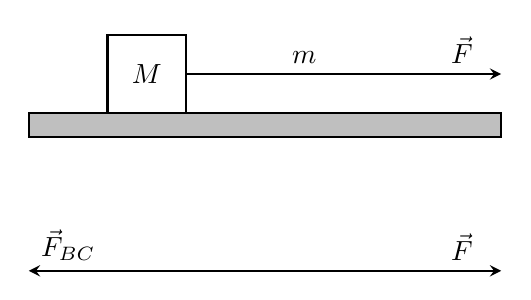
\begin{tikzpicture}[>=stealth,thick]

% Block on surface
\draw[fill=white] (0,0) rectangle (1,1) node[midway] {$M$};
\draw[fill=gray!50] (-1,-0.3) rectangle (5,0); % surface

% Rope and force
\draw (1,0.5) -- (4,0.5);
\draw[->] (4,0.5) -- (5,0.5) node[midway,above] {$\vec{F}$};
\node[above] at (2.5,0.5) {$m$};

% Second diagram (forces on rope)
\draw (0,-2) -- (4,-2);
\draw[->] (4,-2) -- (5,-2) node[midway,above] {$\vec{F}$};
\draw[<-] (-1,-2) -- (0,-2) node[midway,above] {$\vec{F}_{BC}$};

\end{tikzpicture}
\end{shaded}


$(a)$ We know $\vec{F}/m = \vec{a}$, so if we consider the block-rope system 
with mass $\phi = M + m$, 


\begin{equation}
  \vec{a} = \frac{\vec{F}}{\phi} 
\end{equation}

which is all we can say.

$(b)$ The rope of mass $m$ receives two forces: $\vec{F}$, which pulls it to the
right, and from Newton's third law $\vec{F}_{BC}$, which is the force exerted by 
the block on the rope, and which pulls it to the left. So 

\begin{equation}
    \vec{F} + \vec{F}_{BC} = m \vec{a}
\end{equation}

But we know

\begin{equation}
    a = \frac{F}{M + m}
\end{equation}

So 

\begin{equation}
    F + F_{BC} = m \frac{F}{M + m}
\end{equation}

from which follows that 

\begin{equation}
    F_{BC} = F - \frac{mF}{M + m}  = F\left(1 - \frac{m}{M + m} \right)
\end{equation}

But 

\begin{equation}
    1 - \frac{m}{M + m}  = \frac{M+m}{M + m} - \frac{m}{M + m}  = \frac{M}{M + m}
\end{equation}

So we have 

\begin{equation}
    F_{BC} = F\left( \frac{M}{M+m} \right) 
\end{equation}

from which follows that 

\begin{equation}
    F_{BC}/F = M / (M+m)
\end{equation}

\textit{QED}.


\pagebreak 

\begin{shaded}
    \textbf{(4)} An 8kg block $A$ lies on an incline of angle $\alpha =
    \ang{37}$ without friction. It is joined through a rope and polley without
    friction to a block $B$ of mass $m_B = 4$kg. Determine $\vec{a}$ the
    acceleration of the masses and the tension of the ropes when the system is
    left to evolve freely. Create a diagram of the isolated body.
\end{shaded}

The mass $A$ moves only up/down the surface. So if we let $\hat{u}$ be the unit
vector parallel and equidirectional to the surface, 

\begin{equation}
    \sum \vec{F_A} = m_A \vec{a_A} = m_A a_A \hat{u}
\end{equation}

Similarly, 

\begin{equation}
    \sum \vec{F_B} = m_B \vec{a_B} = m_B a_B \hat{j}
\end{equation}

This entails that, in magnitude, 

\begin{equation}
    \left| \sum \vec{F_A} \right|  = m_A a_A, \qquad \left| \sum \vec{F_B}
    \right| = m_B a_B
\end{equation}

But since the objects move under equal and opposite accelerations, $a_A = -a_B$.
So if we define $a := a_A$ as the acceleration of $A$, equation $(25)$ becomes 

\begin{equation}
    \left| \sum \vec{F_A} \right|  = m_A a, \qquad \left| \sum \vec{F_B}
    \right| = m_B (-a)
\end{equation}

Now, let $\theta$ be the angle between $\hat{u}$ and $\vec{W}$ the weight vector
of $A$. Then the projection of $\vec{W}$ along the surface is $W_{\parallel} =
-m_A g \cos \theta$. And since this and the tension of the rope are the only
forces moving $A$ along the surface, we have 

\begin{equation}
    \left|\sum \vec{F_A} \right| = W_{\parallel} + T = -m_A g \cos \theta + T
\end{equation}

Similar reasoning gives that 

\begin{equation}
    \left|\sum \vec{F_B}  \right| = -m_B g + T
\end{equation}

So, combining these last two results with equation $(26)$,

\begin{equation}
    T - m_A g \cos \theta = m_A a, \qquad T - m_B g = m_B (-a)
\end{equation}

Solving $T$ in one of these equations and substituting it into the other, with
$\theta = \ang{90} - \ang{37} = \ang{53}$, $m_A = 8\text{kg}, m_B = 4\text{kg}$,
one readily obtains after a bit of algebra that 

\begin{equation}
    a \approx -0.665 \frac{m}{s^2}
\end{equation}

\pagebreak 

\begin{shaded}
    \textbf{(5)} Dos bloques de masas $m_1$ y $m_2$ están en contacto sobre una mesa
    sin rozamiento. Una fuerza horizontal $\vec{F}$ se aplica sobre el primer
    bloque.

(a) Encuentre la aceleración del sistema y la fuerza de contacto entre los dos
bloques. Evaluar para el caso que $m_1 = 2\text{kg}, m_2 = 1\text{kg}$ y $\left|
\vec{F} \right| = 3N $. 

(b) Muestre que si la misma fuerza $\vec{F}$ se aplica en sentido contrario, es
decir sobre $m_2$ en lugar de $m_1$, la fuerza de contacto será distinta.
Explique realizando un diagrama de cuerpo aislado.
\end{shaded}

$(a)$ Considering the two blocks as a system, the mass of the system is $m_1 + m_2$,
so 

\begin{equation}
    F = (m_1 + m_2)a \Rightarrow a = \frac{F}{m_1 + m_2}
\end{equation}

If $m_1 = 2\text{kg}, m_2 = 1\text{kg}$ and $\left| \vec{F}\right| = 3N$,we have 

\begin{equation}
    a = \frac{3N}{3\text{kg}} = 1\frac{m}{s^2}
\end{equation}

Consider the lone body diagram of $m_2$. The only force exerted on this body is
the contact force $F_c$, so the magnitude of its acceleration is equal to the
magnitude of this force. But its acceleration is equal to the acceleration of
the system (would it make sense for the second block to accelerate at a
different rate than the system?) In short,

\begin{equation}
    F_c = m_2 a = \frac{F m_2}{m_1 + m_2} 
\end{equation}

$(b)$ By the same reasoning as before, if the force were applied leftwards onto
$m_B$, the contact force would be the only thing moving $m_A$, so that 

\begin{equation}
    F_C = m_1 a \neq m_2 a
\end{equation}

at least as long as $m_1 \neq m_2$.

\pagebreak 

\begin{shaded}
    \textbf{(6)} A ball of mass $m = 10\text{kg}$ hangs from a rope on the roof
    of a car. The maximum tension which the rope can take without breaking is
    $500N$. What is the maximal horizontal acceleration which the car can recah
    without the rope breaking? Determine the angle between the rope and the
    vertical for that maximal acceleration.
\end{shaded}

The forces operating on the ball are its weight, which pulls it downard (
$\vec{W} = W \hat{j}$), and the tension of the rope. From Newton's second law, 

\begin{align*}
    \vec{W} + \vec{T} &= m \vec{a} \\ 
    \Rightarrow \vec{T} &= m\vec{a} - \vec{W} \\ 
                        &= ma
    \hat{i} - W \hat{j}
\end{align*}

(since acceleration is strictly horizontal). Furtheremore, we know 

\begin{equation*}
    W = -g10 \text{kg} = -9.8 \frac{m}{s^2} \cdot 10\text{kg} = -98N
\end{equation*}

We are interested in the acceleration which breaks the rope, i.e. which causes a
tension superior to 500$N$. The tension of the rope is 

\begin{align*}
    \left| \vec{T} \right| 
    &= \sqrt{(ma)^2 + W^2} \\ 
    &= \sqrt{100\text{kg}^2 a^2 + 98^2N^2} \\ 
    &= \sqrt{100\text{kg}^2 a^2 + 9604N^2}
\end{align*}

So to find the acceleration which causes the tension to be $500N$, we solve

\begin{align*}
    &500N = \sqrt{100\text{kg}^2 a^2 + 9604N^2} \\ 
    \iff &500^2 N^2 = 100\text{kg}^2 a^2 + 9604N^2 \\ 
    \iff &a = 49.03 \frac{m}{s^2}
\end{align*}

as it is easy to see algebraically. So, the rope breaks if $a \geq 49.03$,
meaning that the rope will not break if the acceleration lies in the open
interval $a < 49.03$. This interval has $49.03$ as supremum, but has no maximum.

$(b)$ The angle between the tension vector $\vec{T}$ and the horizontal is 

\begin{equation*}
    \arctan\left( \frac{T_y}{T_x} \right) 
\end{equation*}

We know $\vec{T} = ma \hat{i} - W \hat{j} = 10\text{kg} a - 98N \hat{j}$. Taking
the maximal acceleration $a = 49.03 m / s^2$, we have $\vec{T} = 490.3N \hat{i}
- 98N \hat{j}$. So the angle between the tension vector and the horizontal is 

\begin{equation*}
    \arctan\left( \frac{98N}{490.3N} \right) = 0.197\text{rad}
\end{equation*}

Now, the angle between $\vec{T}$ and the vertical will be $\ang{90} =
\frac{\pi}{2}\text{rad}$ minus the angle between $\vec{T}$ and the horizontal.
So the angle between $\vec{T}$ and the vertical is 

\begin{equation}
    \frac{\pi}{2}\text{rad} - 0.197\text{rad}= 1.37379633\text{rad}
\end{equation}

\pagebreak 


\begin{shaded}
\textbf{Problem 7.} Three blocks of masses $m_1$, $m_2$, and $m_3$ are connected by strings that sustain tensions $\vec{T}_1$ and $\vec{T}_2$ on a frictionless table. They are pulled by a string attached to $m_3$ with a tension $|\vec{T}_3| = 60~\mathrm{N}$. The strings are massless and inextensible.

\begin{enumerate}
    \item[(a)] Find $\vec{T}_1$ and $\vec{T}_2$ as functions of the block masses.
    \item[(b)] Evaluate (a) for the particular case $m_1 = 20~\mathrm{kg}$, $m_2 = 20~\mathrm{kg}$, and $m_3 = 30~\mathrm{kg}$.
    \item[(c)] Repeat (a) and (b) for the case of vertical motion.
\end{enumerate}

\begin{center}
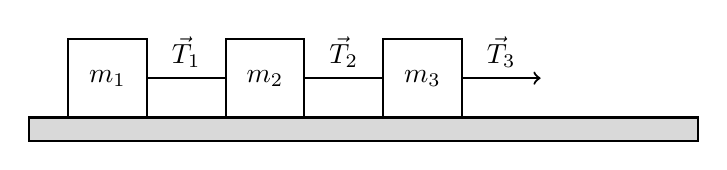
\begin{tikzpicture}[scale=1.0]
    % Draw the table
    \draw[thick, fill=gray!30] (-0.5,0) rectangle (8,0.3);

    % Draw blocks
    \draw[thick, fill=white] (0,0.3) rectangle (1,1.3) node[midway] {$m_1$};
    \draw[thick, fill=white] (2,0.3) rectangle (3,1.3) node[midway] {$m_2$};
    \draw[thick, fill=white] (4,0.3) rectangle (5,1.3) node[midway] {$m_3$};

    % Draw strings and tensions
    \draw[thick] (1,0.8) -- (2,0.8) node[midway, above] {$\vec{T}_1$};
    \draw[thick] (3,0.8) -- (4,0.8) node[midway, above] {$\vec{T}_2$};
    \draw[->, thick] (5,0.8) -- (6,0.8) node[midway, above] {$\vec{T}_3$};
\end{tikzpicture}
\end{center}


\end{shaded}

$(a)$ As always, let us ask: what are the forces at work on each body? The mass
$m_1$ is affected only by $\vec{T_1}$, so

\begin{equation}
    \vec{T_1} = m_1a 
\end{equation}

The mass $m_2$ is affected by $\vec{T_2}$, which pulls it to the right, and
$\vec{T_1}$, which pulls it to the left, so 

\begin{equation}
    \vec{T_2} - \vec{T_1} = m_2 a
\end{equation}

By the same logic, 

\begin{equation}
    \vec{T_3} - \vec{T_2} = m_3 a
\end{equation}

From $(38)$ we have 

\begin{equation}
    \vec{T_3} - m_3a = \vec{T_2} \iff 60N - m_3a = \vec{T_2}
\end{equation}

Substituting this into $(37)$, we have 

\begin{equation}
    60 N - m_3 a - \vec{T_1} =m_2 a \iff 60N - m_3a - m_2 a = \vec{T_1}
\end{equation}

Substituting into $(36)$,

\begin{equation}
    60N - m_3 a - m_2a = m_1 a \iff \frac{ 60N }{m_1 + m_2 + m_3} = a
\end{equation}

Now that we have determined the acceleration $a$ as a function of the masses, 
we have 

\begin{align*}
    T_1 &= \frac{m_1 60N}{m_1 + m_2 + m_3} \\ 
    T_2 &= m_2a + T_1 \\ 
        &= \frac{60Nm_2}{m_1 + m_2 + m_3} + \frac{m_1 60N}{m_1 + m_2
    + m_3} \\ 
        &= 60N \frac{m_1 + m_2}{m_1 + m_2 + m_3}
\end{align*}




\pagebreak 

\begin{shaded}
\textbf{(9)} A block of mass $m$ slides on the floor while a force of magnitude
$|\vec{F}| = 12~\mathrm{N}$ pulls it at an angle $\theta$ with the horizontal.
The coefficient of kinetic friction is $0.4$. The angle $\theta$ can vary
between $0^\circ$ and $90^\circ$, and the block always remains on the floor.
What is the angle $\theta$ that gives the maximum acceleration?
\end{shaded}

The forces acting on the mass are the normal force, its weight (gravity),
$\vec{F}$ and the dynamic friction $\vec{F}_{r.d.}$. Since the object moves only
horizontally, $\vec{a} = a \hat{i}$. So by Newton's second law, 

\begin{equation*}
    \vec{W} + \vec{N} + \vec{F} + \vec{F}_{r.d.} = m a \hat{i}
\end{equation*}

from which follows 

\begin{equation}
    F_{\parallel} + F_{r.d.} = ma
\end{equation}

where $F_\parallel$ is the projection of $F$ parallel to the $x$-axis. We know
$F_{r.d.} = \mu \left| \vec{N} \right| $ where $\mu$ is the dynamic frictoin
coefficient. So we obtain

\begin{equation}
    \left| \vec{F} \right| \cos \theta + \mu_{r.d.} \left| \vec{N} \right| = ma
\end{equation}

Using the information of the exercise, this gives 

\begin{equation}
    12N \cos \theta + 0.4 \left| \vec{N} \right|  = ma
\end{equation}

We must know determine the magnitude of $\vec{N}$, the vertical forces at play.
These are $(a)$ the force that opposes gravity, of magnitude equal to that of
gravity, and the vertical component of $\vec{F}$, which we term $F_\parallel$.
So 

\begin{equation}
    \left| \vec{N} \right| = N = gm_A + 12N \sin \theta
\end{equation}

In conclusion, 

\begin{equation}
    12N \cos \theta + \mu\left( g m_A + 12N \sin \theta \right)  = ma
\end{equation}

Rearranging, 

\begin{equation}
    a = \frac{12N(\cos \theta + \mu\sin \theta) + \mu gm_A}{m}
\end{equation}

This will of course be maximized when $\varphi(\theta) = \cos \theta +
\mu \sin \theta$ is maximized, under the constraint $0 \leq \theta \leq
\pi / 2$. The derivative of $\varphi$ is 

\begin{equation}
    \varphi'(\theta) = -\sin \theta + \mu \cos \theta
\end{equation}

and this derivative is zero if and only if $\sin \theta = \mu \cos
\theta$, which holds if and only if $\frac{\sin \theta}{\cos \theta} = \mu$, or
equivalently $\tan \theta = \mu$. But this holds if and only if 
$\arctan \mu = \theta$. With $\mu = 0.4$, we obtain $\theta \approx 0.380$.

$\therefore $ Acceleration is maximized if $\theta \approx 0.380 \text{rad}
\approx \ang{21.77}$.


\pagebreak 

\begin{shaded}
\textbf{10.} Two masses $m_A$ and $m_B$ slide down an inclined plane, connected
by a massless rope, where $m_A$ pulls $m_B$. The inclination angle is $\alpha$.
The coefficient of kinetic friction between $m_A$ and the plane is $\mu_A$, and
between $m_B$ and the plane is $\mu_B$.  

\begin{enumerate}
    \item[(a)] Find an expression for the tension $\vec{T}$ in the rope that connects $m_A$ and $m_B$, expressed in terms of the problem variables.
    \item[(b)] Find an expression for the acceleration $\vec{a}$ that both bodies have.
    \item[(c)] How do the answers change if instead $m_B$ pulls $m_A$?
\end{enumerate}

\begin{center}
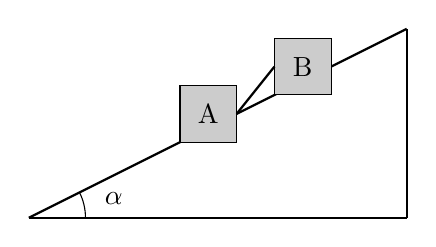
\begin{tikzpicture}[scale=1.2]
  % Inclined plane
  \draw[thick] (0,0) -- (4,0);
  \draw[thick] (0,0) -- (4,2);
  \draw[thick] (4,0) -- (4,2);

  % Blocks
  \draw[fill=black!20] (1.6,0.8) rectangle (2.2,1.4) node[pos=.5] {A};
  \draw[fill=black!20] (2.6,1.3) rectangle (3.2,1.9) node[pos=.5] {B};

  % Rope
  \draw[thick] (2.2,1.1) -- (2.6,1.6);

  % Inclination angle
  \draw (0.6,0) arc[start angle=0,end angle=26.565,radius=0.6];
  \node at (0.9,0.2) {$\alpha$};
\end{tikzpicture}
\end{center}
\end{shaded}

Object $A$ is affected by gravity, the normal force, the tension of the
rope, and friction:

\begin{equation*}
    \sum \vec{F_A} = \vec{T}_A + \vec{N}_A + \vec{W}_A + \vec{R}_A = m_A \vec{a}
\end{equation*}

Let us decompose these forces into components parallel and perpendicular to the
slope. Let $\hat{x'}, \hat{j'}$ be the unit vectors parallel and perpendicular
to the slope, with $\hat{x'}$ going up the slope and $\hat{j}$ with the same
direction as $\vec{N}$.

(Weight.) The angle between $\vec{W_A}$ and $\hat{x}'$ is $\frac{\pi}{2} -
\alpha$, so we readily know that 

\begin{equation}
    W_{A \parallel } = -m_A g \sin \alpha, \qquad W_{A \perp} = -m_A g \cos \alpha
\end{equation}

(Normal.) The normal force will be strictly perpendicular to the incline and
will counteract gravities force:

\begin{equation}
    N_{A \parallel } = 0, \qquad N_{A \perp} = m_A g \cos \alpha
\end{equation}

(Friction.) Friction is parallel to the slope and contrary to the direction of
movement, so it will be directed up the slope. Thus, 

\begin{equation}
    R_{A \parallel} = \mu_A \left| \vec{N} \right| = \mu_A m_A g \cos \alpha,
    \qquad R_\perp = 0
\end{equation}

(Tension.) The tension also has a null perpendicular component, acting only
parallel to the surface. For object $A$, the tension of the rope acts up the
slope and towards object $B$. And from our previous results, it follows  that 

\begin{align}
    &T_{\parallel } + N_{A \parallel } + W_{A \parallel } + R_{A \parallel } = m_A a\\ 
    \iff ~ ~ ~ 
    &T_{\parallel} - m_A g \sin \alpha + \mu_A m_A g \cos \alpha = m_A
    a\nonumber\\
    \iff ~ ~ ~& T_{\parallel } = m_A a + m_A g \sin \alpha - \mu_A m_A g \cos
    \alpha\nonumber
\end{align}

Note that we do not write $T_{A \parallel}$ but simply $T_\parallel$, since the
tension is equal in absolute value for $A$ and $B$, i.e. we may define
$T_\parallel := T_{A \parallel}$ and then simply $T_{B \parallel} =
-T_\parallel$.

Now, the same results follow for object $B$, but of course with its own mass and
friction coefficient. So

\begin{align}
    &-T_\parallel + N_{B \parallel} + W_{B \parallel} + R_{B \parallel} = m_B
    a \\ 
    \iff ~ ~ ~ 
    &-T_\parallel - m_B g \sin \alpha + \mu_B m_B g \cos \alpha = m_B a
    \nonumber
\end{align}

If we add $(52)$ and $(53)$, we see that $T$ disappears and we obtain an
equation with only $a$ unknown: 

\begin{align*}
    &\text{Eq. (52)} + \text{Eq. (53)} \\ 
    \Rightarrow~ ~ ~  
    & ( N_{A\parallel} + W_{A \parallel} + R_{A \parallel} ) + (N_{B \parallel} +
    W_{B \parallel} + R_{B \parallel} )= a(m_A + m_B) \\ 
    \Rightarrow~ ~ ~ 
    & \left( 
        -m_A g \sin \alpha - m_B g \sin \alpha
    \right) + 
    \left( 
        \mu_A m_A g \cos \alpha + \mu_B m_B g \cos \alpha
    \right) = a(m_A + m_B) \\ 
    \Rightarrow ~ ~ ~ 
    &\left( -g\sin \alpha (m_A + m_B) \right) + 
    \left( g \cos \alpha (m_A \mu_A + m_B \mu_B) \right) = a(m_A + m_B) \\ 
    \Rightarrow ~ ~ ~ 
    &-g \sin \alpha + g \cos \alpha ~ \frac{m_A \mu_A + m_B \mu_B}{m_A + m_B} = a
\end{align*}

Now that we know $a$, we may substitute it in the simplified form of equation
$(52)$ to obtain an expression of $T_\parallel =: T$ in terms of the problem
variables: 

\begin{align*}
    &T = m_A a + m_A g \sin \alpha - \mu_A m_A g \cos \alpha \\ 
    \iff ~ ~ ~ 
    &T = m_A \left( a + g \sin \alpha - \mu_A g \cos \alpha \right) \\ 
    \iff ~ ~ ~ 
    &T = m_A 
    \left( 
        -g \sin \alpha + \frac{m_A \mu_A + m_B \mu_B}{m_A + m_B}g \cos \alpha
    + g \sin \alpha - \mu_A g \cos \alpha\right) \\ 
    \iff ~ ~ ~ 
    &T = m_A g \cos \alpha
    \left( \frac{m_A \mu_A + m_B \mu_B}{m_A + m_B} - \mu_A \right) \\
    \iff ~ ~ ~ 
    &T = m_A g \cos \alpha
    \left( \frac{m_A \mu_A + m_B \mu_B - \mu_A(m_A + m_B)}{m_A + m_B}
    \right)\\
    \iff ~ ~ ~ 
    &T = m_A g \cos \alpha
    \left( \frac{m_A \mu_A + m_B \mu_B - m_A \mu_A - m_B \mu_A}{m_A + m_B}
    \right)\\ 
    \iff ~ ~ ~ 
    &T = m_A g \cos \alpha
    \left( \frac{m_B(\mu_B - \mu_A)}{m_A + m_B}
    \right)\\ 
    \iff ~ ~ ~ 
    &T =g \cos \alpha  ~ \frac{m_A m_B( \mu_B - \mu_A )}{m_A + m_B}
\end{align*}

\pagebreak 


\begin{shaded}
\textbf{11.} The spring of a laboratory dynamometer has been stretched 
$11.7 \, \text{cm}$ at the maximum scale, which corresponds to $2 \, N$.

\begin{enumerate}[label=(\alph*)]
    \item What is the spring constant of the spring with which the dynamometer 
    has been manufactured?
    \item How much will it stretch when a force 
    $\lvert \vec{F} \rvert = 0.4 \, N$ is applied to it?
\end{enumerate}
\end{shaded}

Sea $k$ la constante del resorte. Sabemos que la fuerza del resorte es 

\begin{equation}
    \vec{F_k} = -k \Delta \ell
\end{equation}

donde $\ell$ es la distancia entre el extremo y la posición de equilibrio. Ahora
bien, sabemos además que si $\delta \ell = 11.7$cm la fuerza se corresponde con 
$2N$, es decir que bajo este supuesto

\begin{equation}
    N + W + F_k = 2N
\end{equation}

Pero asumimos que $\vec{N} + \vec{W} = 0$, con lo cual $F_k = 2N$, i.e. 

\begin{equation}
    k(11.7 \text{cm}) = 2N
\end{equation}

Por lo tanto, 

\begin{align*}
    k 
    &= \frac{2N}{11.7\text{cm}} \\ 
    &= \frac{2}{11.7} \frac{\text{kg} \cdot
    ms^{-2}}{cm} \\ 
    &=\frac{2}{0.117} \frac{N}{m}
\end{align*}

\pagebreak 

\begin{shaded}
\textbf{Problema 12.}  
Dos resortes de longitudes naturales $L_0 = 0.5 \, \text{m}$ pero con diferentes constantes 
elásticas, $K_1 = 50 \, \text{N/m}$ y $K_2 = 100 \, \text{N/m}$, se encuentran colgados del 
techo. Un cuerpo de masa $m = 2.5 \, \text{kg}$ que inicialmente está suspendido de ellos es 
estirado hacia abajo hasta que la longitud de los resortes se duplica. ¿Cuál es la aceleración 
$\vec{a}$ que adquiere el cuerpo cuando se deja libre? \\[1em]

% --- TikZ Diagram ---
\begin{center}
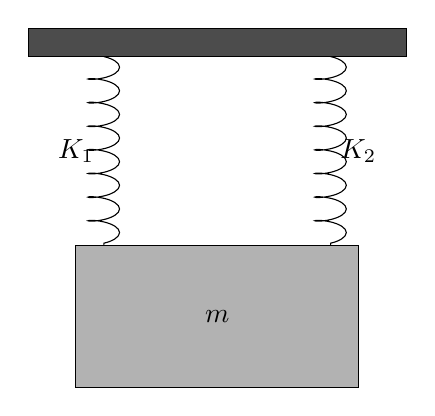
\begin{tikzpicture}[scale=1.2]

% Ceiling
\draw[fill=black!70] (-2,0) rectangle (2,0.3);

% Springs
\draw[decoration={coil,aspect=0.3,segment length=3mm,amplitude=2mm},decorate] (-1.2,0) -- (-1.2,-2);
\draw[decoration={coil,aspect=0.3,segment length=3mm,amplitude=2mm},decorate] (1.2,0) -- (1.2,-2);

% Labels for springs
\node[left] at (-1.2,-1) {$K_1$};
\node[right] at (1.2,-1) {$K_2$};

% Mass block
\draw[fill=black!30] (-1.5,-2) rectangle (1.5,-3.5);
\node at (0,-2.75) {$m$};

\end{tikzpicture}
\end{center}
\end{shaded}

The acceleration of the body is strictly vertical, i.e. $\vec{a} = a \hat{j}$
for some $a \in \mathbb{R}$. Both springs will exert a force on the object, and
this force will also be strictly vertical. In particular, the forces acting on
the body when it is at a distance $\Delta \ell$ from the point of equilibrium
are 

\begin{equation*}
    \vec{F_1} = -K_1 \Delta \ell ~ \hat{j}, \qquad \vec{F_2} = -K_2 \Delta \ell
    ~ \hat{j}, \qquad \vec{W} =
    -gm ~ \hat{j}
\end{equation*}

It follows that 

\begin{align*}
    &-K_1 \Delta \ell - K_2 \Delta \ell - gm = ma \\ 
    \Rightarrow 
    &-\Delta \ell(K_1 + K_2) - gm = ma \\
    \Rightarrow 
    &-\Delta \ell(150 \text{N / m}) - gm = ma \\
\end{align*}

Since in the conditions described the length of the springs is doubled, going
from $0.5\text{m}$ to $1\text{m}$, the mass will be at a distance of
$-0.5\text{m}$ from its resting position. So we will have 

\begin{align*}
    &\frac{1}{2}\text{m} \left( 150 \text{N/m} \right)  - gm = ma \\ 
    \Rightarrow ~ ~ ~
    &75N - gm = ma \\ 
    \Rightarrow ~ ~ ~ 
    &\frac{75N}{2.5\text{kg}} - g = a \\ 
    \Rightarrow ~ ~~ 
    &30ms^{-2} - 9.8 ms^{-2} = a
\end{align*}

So $a = 20.2 ms^{-2}$.


\pagebreak 

\begin{shaded}
    \textbf{(13)} A spring with constant $k$ has an extreme fixed adn the other
    coinciding with coordinate $x_0$ when there is nodeformation. A mass $m$
    lies at this extreme, is displaced to position $x_1$, and let go from that
    position. Assume $k = 8 \text{N/m}$, $m = 2\text{kg}, x_0 = 40\text{cm}, x_1
    = 55\text{cm}$. 

    $(a)$ Determine $x(t), v(t), a(t)$ and plot them. 

    $(b)$ Determine the period, frequency, and extreme coordinates of the
    movement, as well as the module of the velocity of $m$, at the point of
    equilibrium.
\end{shaded}

Recordemos que

\begin{equation*}
    a(t) = -\omega^2 x(t), \qquad v(t) = \omega A \cos(\omega t + \phi), \qquad
    x(t) = x_0 + A \sin(\omega t + \phi)
\end{equation*}

con $\omega = \sqrt{k / m}$ y con $x(t)$ el desplazamiento de la masa, en el
tiempo $t$, respecto a la posición de equilibrio. Dado que $x(0) = x_1, v(0) =
0$, tenemos 

\begin{equation*}
    \omega A \cos(\phi) = 0, \qquad A \sin(\phi) = x_1 - x_0
\end{equation*}

Como $x_1 \neq 0$, tenemos que $A \neq 0, \sin(\phi) \neq 0$, de lo cual se
sigue que $\phi \neq 0$. Por ende, en la ecuación $\omega A \cos(\phi) = 0$,
dado que $\omega \neq 0$, debe satisfacerse $\cos(\phi) = 0$, es decir $\phi =
\frac{\pi}{2}$. Usando este resultado en la ecuación de la derecha, vemos que 

\begin{equation*}
    A \sin\left( \frac{\pi}{2} \right) = x_1 - x_0 \iff A = x_1 - x_0 =
    15\text{cm}
\end{equation*}

Tomando 

\begin{equation*}
    \omega = \sqrt{\frac{k}{m}}  = \sqrt{\frac{8\text{N}}{2\text{kg m}}} =
    2\frac{ms^{-1}}{m} = 2s^{-1}
\end{equation*}

obtenemos 

\begin{equation*}
    x(t) = 40\text{cm} + 15\text{cm}\sin\left( 2s^{-1} \cdot t + \frac{\pi}{2} \right) 
\end{equation*}


\begin{equation*}
    a(t) = 2s^{-1} \cdot 15\text{cm} \cdot \cos \left( 2s^{-1} \cdot t +
    \frac{\pi}{2} \right) 
\end{equation*}

etc. Simplificar unidades (e.g. $a(t)$ queda todo en cm sobre segundos, etc.)

$(b)$ El periodo es $T = \frac{2\pi}{\omega} = \frac{2\pi}{2s^{-1}} =
\pi\text{s}$. La frequencia es la inversa del periodo, i.e. $F =
\frac{1}{\pi\text{s}} \frac{1}{\pi}\text{Hz}$.

\pagebreak 

\section{P3}


\begin{shaded}
\textbf{1.} Una masa pequeña se coloca en el extremo de una cuerda de largo 
$L = 132 \, \text{cm}$ y se suelta desde el reposo, siendo $\theta_A = 5$ 
(posición A). Sabiendo que $d = 66 \, \text{cm}$, determinar:

\begin{enumerate}[label=(\alph*)]
    \item El valor de la velocidad en el punto más bajo de la trayectoria 
    (posición B).
    \item El valor de $\theta_C$ para la máxima altura que alcanza la masa 
    (posición C).
    \item La tensión de la cuerda en la posición B.
\end{enumerate}


\end{shaded}

En el sistema de coordenadas que elegí, 

\begin{equation*}
    A 
    &= L \cos \theta ~ \hat{i} + L \sin \theta ~ \hat{j}, \qquad B =
    132\text{cm} ~ \hat{i}
\end{equation*}

La distancia vertical en el espacio físico se corresponde con la distancia
horizontal en mi sistema de coordenadas, y se obtiene que la distancia vertical
(física) entre $A$ y $B$ es 

\begin{equation}
    \Delta h = B_x - A_x \approx 0.51\text{cm}
\end{equation}

Recordemos que la energía kinética (en un momento dado) y la energía potencial
son:

\begin{equation*}
    K = \frac{1}{2} m v^2, \qquad U = mg\Delta h
\end{equation*}

donde $\Delta h$ es la altura del objeto y $E = U + K$. 

Tomemos como momento inicial el instante en que el objeto se suelta desde el
reposo, y como momento final el instante en que el objeto ocupa el punto $B$.
Pues la velocidad en el instante cero es cero, 

\begin{equation*}
    E_0 = K_0 + U_0 = 0 + mg \Delta h = mg \Delta h
\end{equation*}

En otras palabras, en el instante cero, la energía se corresponde con la energía
potencial, pues el objeto está en reposo con altura $\Delta h$. Ahora bien, de
manera análoga,

\begin{equation*}
    E_f = K_f + U_f = \frac{1}{2} m v_f^2 + 0 = \frac{1}{2}mv_f^2
\end{equation*}

donde $v_f$ es la velocidad en el instante en que el cuerpo ocupa el punto $B$.
En otras palabras, en este caso, la energía se corresponde enteramente con la
energía kinética. Por preservación de la energía, $E_f = E_0$, y por lo tanto
obtenemos:

\begin{equation}
    mg \Delta h = \frac{1}{2}mv_f^2
\end{equation}

lo cual implica que $v_f = \sqrt{2g \Delta h} $. Aproximando $g \approx 9.8
\frac{m}{s^2}$ y $\Delta h \approx 0.51\text{cm}$, obtenemos 

\begin{align*}
    v_f 
    &= \sqrt{2 \cdot 9.8 \frac{\text{m}}{\text{s}^2} \cdot 0.0051 \text{m}}\\ 
    &\approx 0.316 \text{m}/\text{s}
\end{align*}

$(b)$ En el instante $t_C$ en que el péndulo se detiene alcanzando el punto $C$,
toda la energía es potencial. Pero por preservación de la energía, $E_C = E_f$.
Como $E_c = U_C$ (la energía es estrictamente potencial), y $E_f = K_f$ (la
energía es estrictamente kinética), obtenemos $E_C = K_f$, es decir

\begin{equation}
    mg \Delta h' = \frac{1}{2} mv_f^2
\end{equation}

donde $\Delta h' = B_x - C_x$ es la distancia vertical (en el espacio físico) entre $C$ y
$B$. Ahora bien, de la ecuación anterior se deduce 

\begin{equation}
    \Delta h' = \frac{1}{2g} v_f^2
\end{equation}

donde conocemos $v_f^2$ por el punto $(a)$. Ahora bien, notemos que en nuestro
sistema de coordenadas, la posición en el eje $x$ del punto $C$ se corresponde
con 

\begin{equation}
    C_x = \cos \theta_C \left| C \right| + d
\end{equation}

con $\left| C \right| = L - d$. Luego 

\begin{equation}
    &C_x = \cos \theta_C (L-d) + d \\
\end{equation}

Por lo tanto, combinando $(6)$ y $(4)$, obtenemos 

\begin{align*}
    &\frac{1}{2g}v^2_f = B_x - \cos \theta_C (L - d) - d\\ 
    \Rightarrow ~ ~ ~ 
    &-\frac{ \frac{1}{2g}v_f^2 - B_x + d }{L - d} = \cos \theta_C
\end{align*}

Es fácil ver que 

\begin{equation*}
    \frac{1}{2g} v_f^2 \approx \frac{0.316^2}{19.6}
    \frac{\frac{m^2}{s^2}}{\frac{m}{s^2}} = 0.005\text{m} =  0.5\text{cm}
\end{equation*}

y que $-B_x + d = (-132 + 66)\text{cm} = -66\text{cm}, L - d = 66\text{cm}$.
Luego obtenemos 

\begin{align*}
    &- \frac{0.5\text{cm} - 66\text{cm}}{66\text{cm}} = \cos \theta_C\\ 
    \Rightarrow ~ ~ ~ 
    & \frac{65.5}{66}\text{cm} = \cos \theta_C \\ 
    \Rightarrow ~ ~ ~ 
    &0.992 \text{cm} = \cos \theta_C
\end{align*}

Como $\cos^{-1}(0.992) = 0.126\text{rad}$, obtenemos que $\theta_C =
0.126\text{rad}$.

$(c)$ Se nos pide la tensión de la cuerda. Recordemos que en un movimiento
pendular como éste, la velocidad angular en el punto de equilibrio es cero.
Recordemos que la aceleración centrípeta es 

\begin{equation}
    a_c = \frac{v^2}{L}
\end{equation}

y por ende la segunda ley de Newton nos dice

\begin{equation}
    T - W = ma_c
\end{equation}

donde $T$ es la tensión de la cuerda (vertical y positiva hacia arriba), $W$ es
la gravedad (vertical y negativa hacia abajo). Por lo tanto, 

\begin{equation}
T - W = m \frac{v^2}{L} \iff T = m \frac{0.316^2 \text{m}^2/\text{s}^2}{L} + mg
\end{equation}

Como $L$ está en centímetros, $\frac{L}{100} \text{m}$ se corresponderá con la
longitud de la soga en metros, y el término izquierdo quedará en metros sobre
segundos cuadrados. Se obtiene entonces 

\begin{equation}
    T \approx m \frac{ 0.099 }{1.32} \frac{\text{m}}{s^2} + m 9.8 \frac{\text{m}}{s^2} = m\left(
    9.875 \text{m}/\text{s}^2 \right) 
\end{equation}

\pagebreak 

\begin{shaded}
    
\textbf{2.} Un bloque de $20 \, kg$ es empujado sobre una superficie horizontal, 
por medio de una fuerza $\vec{F}$ que forma un ángulo $\theta$ con ésta 
(ver figura). Durante el movimiento la fuerza aumenta de acuerdo con la 
relación $|\vec{F}(x)| = 6x \, N$.

\begin{enumerate}
    \item[(a)] Calcule el trabajo realizado por esta fuerza mientras el cuerpo 
    se desplazó en línea recta desde $x = 10 \, m$ hasta $x = 20 \, m$.
    
    \item[(b)] Calcule la energía cinética del cuerpo en la posición final, 
    asumiendo que se parte del reposo. Considere dos casos: 
    \begin{enumerate}
        \item[(i)] $\mu_d = 0$
        \item[(ii)] $\mu_d = 0.05$
    \end{enumerate}
\end{enumerate}

\end{shaded}

$(a)$ Recordemos que el trabajo realizado por una fuerza $\vec{F}$ al desplazar
un cuerpo con un desplazamiento $\Delta \vec{r}$ es el producto punto de ambos
vectores: 

\begin{equation}
    W = \left| F \right| \cdot \left| \Delta \vec{r} \right| \cdot \cos \theta
\end{equation}

con $\theta$ el ángulo entre ambos vectores. En el caso de un movimiento
horizontal, como el problema, $\Delta \vec{r} = \Delta x \cdot \hat{i}$  y por
lo tanto escribimos simplemente $W = F \cdot \Delta x \cdot \cos \theta$. Notar
que si la fuerza y el desplazamiento tienen la misma dirección, $\cos \theta =
1$ y $W = F \Delta x$, y si la fuerza y el desplazamiento tienen dirección
opuesta, $\cos \theta = -1$ y $W = -F \Delta x$ (es decir, la fuerza hace un
trabajo negativo).

En nuestro problema, la magnitud $\vec{F}$ es variable respecto a la posición
$x$. Por lo tanto, debemos integrar la expresión para la fuerza en cada una de
las posiciones tomadas por el cuerpo:

\begin{equation*}
    W_F 
    = \int_{x = 10\text{m}}^{x=20\text{m}} \left| \vec{F}(x) \right| \cos \theta ~ dx
    = 6\text{N} \cos \theta \int_{x = 10\text{m}}^{x=20\text{m}} x ~ dx = 900
    \cos \theta ~ \text{J}
\end{equation*}

(Notar, si esto no es claro, que $dx$ es un desplazamiento infinitesimalmente
pequeño. Es decir que la expresión siendo integrada sigue siendo exactamente de
la forma de la ecuación 11: magnitud de la fuerza por magnitud del
desplazamiento por ángulo entre ambos, i.e. producto punto).

\pagebreak 

$(b)$ Recordemos que $W = \Delta K$. A su vez, $W = W_F + W_R$ con $W_F$ el
trabajo de la fuerza $\vec{F}$ y $W_R$ el trabajo de la fuerza de rozamiento
$\vec{R}$. En términos generales, asumiendo un coeficiente de rozamiento
dinámico $\mu_d$ arbitrario,

\begin{equation*}
    W_R = \left| \vec{R} \right| \Delta x \cos \varphi = \mu_d \left| \vec{N} \right|
    \Delta x \cdot \cos \varphi
\end{equation*}

donde $\varphi$ el ángulo entre la dirección del movimiento y la fuerza de
rozamiento. Pero la fuerza de rozamiento se opone al movimiento, i.e. su ángulo
es 180 grados y $\cos \varphi = \cos \ang{180} = -1$. La fuerza normal tiene
magnitud equivalente a la magnitud de la gravedad. Luego 

\begin{equation*}
    W_R = -\mu_d mg \cdot \Delta x = -\mu_d 1960 \text{J}
\end{equation*}

Por ende, 

\begin{equation*}
    W = W_R + W_F = 900 \cos \theta \text{J} - \mu_d 1960\text{J}
\end{equation*}

Entonces 

\begin{equation*}
    \Delta K = 900 \cos \theta \text{ J} - \mu_d 1960 \text{ J}
\end{equation*}

Pero la velocidad inicial es cero, así que $\Delta K = K_f$ la energía kinética
final. Con lo cual

\begin{equation*}
    K_f = ( 900\cos \theta - \mu_d 1960 ) \text{ J}
\end{equation*}

Sustituyendo con $\mu_d = 0, \mu_d = 0.05$ se obtienen las respuestas.


\begin{shaded}
    \textbf{(3)} A 1kg mass is left to slide down a plane with a $\theta =
    \ang{30}$ angle with respect to the horizontal and from a height of 1m. 

    $(a)$ Find the velocity of the block when it reaches the floor, assuming no
    friction.

    $(b)$ Same but assuming $\mu_d = 0.3$.

    $(c)$ Compare the value of $(a)$ with the value obtained if the block is
    dropped in free fall from the same height. 

    $(d)$ For $(b)$, compute the loss of energy.
\end{shaded}

$(a)$ Recall that $K = \frac{1}{2}m v^2$ and that $W = \Delta K$. 
Since the
projection of the weight vector along the incline is $P_\parallel = mg \sin
\theta$,

\begin{equation}
    W = P_{\parallel} \Delta x'
\end{equation}

where $\Delta x'$ is the change of position in terms parallel to the incline.
The incline is the magnitude of a vector $\vec{h}$ with $y$-coordinate 1m and
angle $\theta$, i.e. $\Delta x' = \left| \vec{h} \right| $. Here, we recall 

\begin{equation*}
    h_x = \left| \vec{h} \right| \cos \theta, \qquad h_y = \left| \vec{h}
    \right|  \sin \theta
\end{equation*}

From the LHS and the fact that $h_y = 1\text{m}$,

\begin{equation*}
    \Delta x' = \left| h \right| = \frac{1\text{m}}{\sin \theta}
\end{equation*}

In short, substituting in $(13)$ with $(14)$,

\begin{equation}
    W = mg \sin \theta \cdot \frac{1\text{m}}{\sin \theta} = mg \text{m} =
    1\text{kg} \cdot 9.8 \frac{\text{m}}{\text{s}^2} \cdot 1\text{m} =
    9.8\text{N} \cdot 1 \text{m} = 9.8 \text{J}
\end{equation}

The velocity at the initial instant is zero, and at the final instant is
unknown, but since $W = \Delta K$ we have 

\begin{align*}
    &W = K_f - K_0 \\ 
    \iff ~ ~ ~
    &9.8\text{J} = \frac{1}{2}m v_f^2 \\ 
    \iff ~ ~ ~ 
    &\frac{ 19.6\text{J} }{1\text{kg}} = v_f^2 \\ 
    \iff ~ ~ ~ 
    &19.6 \frac{\text{m}^2}{\text{s}^2} = v_f^2 \\ 
    \iff ~ ~ ~ 
    &\sqrt{19.6 \frac{\text{m}^2}{\text{s}^2}}  = v_f \\
    \iff ~ ~ ~ 
    &4.42718872424 \frac{\text{m}}{\text{s}}  = v_f 
\end{align*}

$(b)$ If we assume there is friction with $\mu_d = 0.3$, then $\vec{R}$ will
oppose the sliding movement with magnitude $\mu_d \left| \vec{N} \right| $. The
magnitude of the normal force balances the perpendicular component of the
weight, i.e. $\left| \vec{N} \right| = P_\perp = mg \cos \theta$. So now the
total work is 

\begin{align*}
    W &= ( P_\parallel - R)\Delta x' \\
    &= \left( mg \sin \theta - \mu_d ~ mg \cos
    \theta \right) \frac{1\text{m}}{\sin \theta}\\ 
    &=mg ~ \text{1m} - \mu_d ~ mg \frac{\cos \theta}{\sin \theta} ~ \text{1m} \\ 
    &= 1\text{m} ~ mg \left( 1 - \mu_d \cot \theta \right)  \\ 
    &= 9.8\text{J}\left( 1 - 0.3 \cdot \sqrt{3}  \right)  \\ 
    &= 9.8\text{J} \cdot 0.480384758 \\ 
    &= 4.70777063\text{J}
\end{align*}

Having found the work, we again use that $W = K_f$ in this scenario to obtain 

\begin{equation}
    4.70777063\text{J} = \frac{1}{2}mv_f^2 \iff\sqrt{9.41554126
    \frac{\text{m}^2}{s^2}} = v_f 
\end{equation}

which gives $v_f = 3.06847539668 \text{m/s}$.

$(c)$ If the object is let to fall freely from one meter, we have 

\begin{equation*}
    W = mg ~ \text{1m}
\end{equation*}

which entails 

\begin{equation*}
    v_f = \sqrt{2 \cdot g ~ 1 \text{m}} = 4.42718872424 \frac{\text{m}}{\text{s}}
\end{equation*}

So interestingly, at the final instant, the velocity of the object if left to
slide coincides with the velocity of the object is left to fall.

\pagebreak 

\begin{shaded}
    \textbf{(4)} A mass of 1kg compresses a spring of constant $k = 2
    \text{N/m}$ over a horizontal surface without friction. The spring is
    compressed 0.3m with respect to its equilibrium position. In a given moment,
    it is released. The mass is not tied to the spring.

    $(a)$ Explain what happens when the spring is released. 

    $(b)$ Compute the work done by the spring. 

    $(c)$ Compute the final velocity which the object raches after being
    released. 

    $(d)$ At the moment when the body is released, it makes contact with a
    surface with friction and $\mu_d = 0.2$. Explain what happens, and the work
    done by the force of friction when the mass reaches half the velocity which
    it carried at the moment of release. 

    $(c)$ Compute the distance the body travels before stopping.
\end{shaded}


\small
\begin{quote}

$(\dagger)$ I misunderstood the statement of the problem and used $y$ instead of
$x$ coords. I'm lazy and will not change it. Just think of $y$ as $x$.

\end{quote}
\normalsize


$(a)$ When the spring is released, the potential energy of the spring becomes
kinetic energy, and there's a transfer of energy from the spring unto the mass.


The mass is pushed away in horizontal and positive direction with the force
transfered by the spring, becoming immediately affected by gravity.

$(b)$ The work done by the spring will correspond to 

\begin{equation*}
    W_R = \int_{x_0}^{x_f} |\vec{R}(x)| ~ dx
\end{equation*}

where $y_0 = y_e - 0.3\text{m}$ and $y_f$ is the point at which the mass stops
making contact with the spring. Theoretically, $y_f$ will correspond to the
point at which the spring stops exerting force unto the mass, i.e. when $\left|
\vec{R}\right| = 0$. Since, by virtue of Hooke's law, $\left| \vec{R} \right| =
-k\Delta y$, it will be zero exactly at $y_e$.

Since the movement of the spring is strictly vertical, $d\vec{y} = dy$. The
magnitude of the force at an arbitrary point $y$ is $-k\Delta y$,
and if we set the origin of our coordinate system precisely at the equilibrium
$y_e$ then $\Delta y = y $. From this follows that 

\begin{equation*}
    W_R = \int_{y_0}^{y_f} \vec{R}(y) ~ dy = \int_{y_0}^{y_f} -k y ~
    ~ dy 
        = -k ~ \frac{y^2}{2}\Big]_{y_0}^{y_f} =
    \frac{k}{2} (y_0^2 - y_f^2)
\end{equation*}

So, 

\begin{equation}
W_R = \frac{2\text{N}}{2\text{m}}\left( -0.3^2\text{m}^2 \right) = 0.09\text{Nm}
= 0.09\text{J}
\end{equation}

$(c)$ We are asked to compute $v_f$ the final velocity reached by the mass after
being released. Recall that 

\begin{equation*}
    W = \Delta K, \qquad K_f = \frac{1}{2}m v_f^2
\end{equation*}

Knowing that $K_0 = 0$, we obtain $W = K_f$, i.e. 

\begin{equation*}
    0.09\text{J} = \frac{1}{2} ~ \text{1kg} ~ v_f^2
\end{equation*}

from which follows 

\begin{equation*}
     \sqrt{\frac{ 2 \cdot 0.09\text{J}  }{\text{kg}}}   = v_f
\end{equation*}

Solving, $v_f = 0.42426406871 \frac{m}{s}$.

$(d)$ Upon making contact with the frictioning surface, friction will exert a
force contrary to the direction of movement, reducing the acceleration of the
object. 

Let $y_*$ be the point at which the object has lost half of its velocity, i.e.
the point at which $v_* = \frac{1}{2} v_f$. (We still use $v_f$ as the velocity
of the object when it loses contact with the spring.) The work of friction, like
any other work, obeys

\begin{align*}
    W_F &= \Delta K \\ 
    &= K_* - K_f\\ 
    &= \frac{1}{2} m v_*^2 - \frac{1}{2}mv_f^2 \\ 
    &= \frac{1}{2}m \left( \frac{1}{2} v_f \right)^2 - \frac{1}{2}m v_f^2 \\ 
    &= \frac{1}{8}m v_f^2 - \frac{1}{2}m v_f^2 \\ 
    &= mv_f^2\left( \frac{1}{8} - \frac{1}{2} \right) \\ 
    &= mv_f^2 \left(  -\frac{3}{8} \right) \\ 
    &= \text{1kg} \cdot 0.18 \frac{\text{m}^2}{\text{s}^2} \cdot -\frac{3}{8} \\ 
    &= \left( 0.18 \cdot -\frac{3}{8} \right) \text{J} \\ 
    &= -0.0675 \text{J}
\end{align*}

$(e)$ When the object stops, its velocity is zero. When the object leaves the
spring, its velocity is $v_f$, as computed before. Therefore, $W = \Delta K =
K_s - K_f = -K_f$, with $W$ the work of all the forces involved in moving the
object across its path.

That said, $W = \left| F \right|\Delta y $, with $F$ the magnitud of all forces
involved in moving the object across its path. From this follows that $-K_f =
\left| F \right| \Delta y$, i.e. $\Delta y = -\frac{K_f}{\left| F \right| }$. So
we have obtained an expression for the distance travelled.

Now, once the object leaves the spring, the only force which contributes to its
movement is the friction of the surface, which acts to stop it. So in fact $F =
R$ the magnitud of friction. We know this magnitud is $-\mu_D \left| \vec{N}
\right| $, and here $\left| \vec{N} \right| = mg$, counteracting gravity.

\begin{align*}
    \Delta y 
    &= - \frac{K_f}{\mu_D m g} \\ 
    &= \frac{\frac{1}{2} m v_f^2}{(0.2) \cdot m \cdot 9.8 \text{m/s}^2} \\ 
    &= \frac{5}{2} \cdot \frac{1}{9.8 \text{m/s}^2} \cdot 0.18( \text{m/s} )^2 \\ 
    &= 0.04591836734 \cdot \frac{\text{m}^2}{\text{s}^2} \cdot
    \frac{\text{s}^2}{\text{m}} \\ 
    &= 0.04591836734 ~ \text{m} \\ 
    &= 4.591836734~ \text{cm}
\end{align*}


\pagebreak 

\begin{shaded}
    \textbf{(5)} A mass of $m = 5$kg is gently layed upon a spring of constant
    $k = 2 \text{N/m}$, which is vertically placed over a horizontal surface. 

    $(a)$ Describe what happens. 

    $(b)$ Compute the work done by the spring when the body reaches equilibrium. 

    $(c)$ Assume the body falls freely from a height of $h = 1\text{m}$ before
    hitting the spring. Compute how much the spring compresses from its
    equilibrium position.
\end{shaded}

$(a)$ When the mass is gently placed upon the object, the force of gravity acts
downard pressing the spring. When the spring is displaced from equilibrium, it
exerts an upward, contrary force which seeks to restore equilibrium. 

$(b)$ The body will reachequilibrium when the magnitude of the forces acting
upon it becomes zero. The two forces acting upon the object are gravity and 
the spring's force. In other words, the body will reach equilibrium if and when 

\begin{equation*}
    -mg = k \Delta y \iff -\frac{5 \text{kg} \cdot 9.8 \text{m/s}^2}{2 \text{N/m}}
    = \Delta y \iff \Delta y = -24.5 \text{m}
\end{equation*}

$\therefore $ The object reaches a state of equilibrium when displaced 24.5
meters below the spring's resting point.

The work exerted by the spring upon the objece is non-constant and therefore 

\begin{align*}
    W_R &= \int_{y=0}^{y=\Delta y} F_R(y) ~ dy \\ 
        &= \int_{y=0}^{y = \Delta y} -ky ~ dy \\ 
        &= -k ~ \frac{y^2}{2}\Big]_{0}^{\Delta y} \\ 
        &= -k \left( \frac{( -24.5\text{m} )^2}{2}\right)  \\ 
        &= -2 \frac{\text{N}}{\text{m}} (300.125\text{m}^2) \\ 
        &= -600.25 \text{J}
\end{align*}

$(c)$ What is the energy of our system in the initial setting? The mass will
begin to fall immediately, but at the initial instant it stands with zero
velocity and only potential energy $U_m^2 = mg \Delta h$. Since the spring is at
equilibrium, its energy is zero.


\small
\begin{quote}

\textbf{Note.} Recall that the potential energy of a spring is $U_R =
\frac{k}{2} x^2$ with $x$ its distance from equilibrium.

\end{quote}
\normalsize

In short, 

\begin{equation*}
    E_0 = mg \Delta h
\end{equation*}

At the final state, the mass has compressed the spring to a maximum distance
from equilibrium, standing still. Since it stands still, its velocity is zero
and therefore so is its kinetic energy. Its potential energy will be 
$U_m^f = mg \Delta h'$ with $\Delta h'$ its distance from equilibrium in the
final state. On the other hand, the spring will now be compressed and still,
thereby containing potential energy $U_R^f = \frac{k}{2}\Delta h'$. So 

\begin{equation*}
    E_f = mg\Delta h' + \frac{k}{2}( \Delta h' )^2
\end{equation*}

Due to preservation of energy, we have 

\begin{equation*}
    mg \Delta h = mg \Delta h' + \frac{k}{2}(\Delta h')^2
\end{equation*}

Now, if the origin of our system is at the equilibrium position, $\Delta h =
\text{1}m$ and $\Delta h' := x$ is unknown, producing the equation 

\begin{align*}
    mg = mgx + \frac{k}{2}x^2 
    \iff~ ~ ~ 
    &\frac{k}{2}x^2 + mgx - mg = 0 \\ 
    \iff ~ ~ ~  
    &\frac{k}{2\phi}x^2 + x - 1 = 0
\end{align*}

with $\phi := mg = 49\text{N}$. So we found a quadratic equation with solutions

\begin{equation*}
    x = \frac{\phi}{k} \left( -1 \pm \sqrt{1 + \frac{2k}{\phi}}  \right) 
\end{equation*}

Now suffices to see that 

\begin{equation*}
    \frac{\phi}{k} = \frac{ 49 }{2} = 24.5 
\end{equation*}

from which follows that $2k / \phi = 2 \cdot \left(\frac{1}{24.5}
\right) = 0.08163265306$. So we obtain 

\begin{equation*}
    x = 24.5 \left( -1 + \sqrt{1.08163265306}  \right) = 24.5 \left(
    0.04001569846 \right) = 0.98038461227
\end{equation*}

Since $x$ is by definition in units of meters, we have found that  
$x = \Delta h' \approx 0.98\text{m} $. So the spring is compressed approximately
0.98 meters below its equilibrium point by the free falling mass.

\pagebreak 

\begin{shaded}
    \textbf{(6)} Un embalaje de masa $m = 250$kg está colgado de un cable de
    largo $L = 10$m. Se lo mueve hacia un lado apartándolo de la vertical una
    longitud $l = 1$m y se lo sostiene allí.

    $(a)$ ¿Cuál es la fuerza necesaria para mantener el embalaje en esa
    posición? 

    $(b)$ ¿Se hace trabajo para sostenerlo allí? 

    $(c)$ ¿Se hizo trabajo para moverlo de lado? ¿Cuánto? 

    $(d)$ La tensión del cable, ¿efectúa algún trabajo?
\end{shaded}

$(a)$ Sea $F_l$ la fuerza necesaria para mantener el embalaje una longitud $l =
1$m a la izquierda. El embalaje es afectado por la gravedad (en su componente
angular) y la tensión del cable, que son fuerzas paralelas y opuestas en
dirección.

Notemos que al desplazar el objeto a la izquierda, su movimiento describe un
arco y la soga termina formando un ángulo $\theta$ respecto a la vertical,
satisfaciendo:

\begin{equation*}
    L  \sin \theta = l \iff \sin \theta = \frac{l}{L} \iff \theta =
    \arcsin\left( \frac{1}{10} \right) 
\end{equation*}

La tensión del cable apunta hacia el origen del cable satisfaciendo 

\begin{equation*}
    T_x = T \sin \theta, \qquad T_y = T \cos \theta
\end{equation*}

Como el objeto está en equilibrio, el componente horizontal de la tensión debe
contrarrestar el componente horizontal de la fuerza $F_l$, y el componente
vertical debe contrarrestar la gravedad. Es decir, $T_x = F_l, T_y = mg$.  Pero 

\begin{equation*}
    T_y = mg \Rightarrow mg = T \cos \theta \Rightarrow T = \frac{mg}{\cos \theta}
\end{equation*}

de lo cual se sigue que 

\begin{equation*}
    F_l = T_x = T \sin \theta = \frac{mg}{\cos \theta} \sin \theta = mg \tan \theta
\end{equation*}

$\therefore $ La magnitud de la fuerza que mantiene al objeto en la posición es
$mg \tan \theta$, y como dicha fuerza solo tiene un componente horizontal, esto
la define completamente.


$(b)$ No. El trabajo de cualquier fuerza involucrada será la magnitud de dicha
fuerza por el desplazamiento del cuerpo. Pero estamos asumiendo que el cuerpo
está sostenido en un punto fijo, i.e. su desplazamiento es cero.

$(c)$ El trabajo realizado para moverlo es dado por $W = \Delta K = \Delta U$,
puesto que en el momento inicial y final la energía kinética es cero. La energía
potencial del objeto es dada por $mg \Delta h$ con $\Delta h$ la altura
alcanzada por la masa (asumiendo que en el reposo la altura es cero).

Del mismo modo que $L \sin \theta$ describe la distancia horizontal que recorre
el objeto respecto al punto en que el cable está colgado, $L \cos \theta$
describe la distanca vertical (respecto a dicho punto). Se sigue que 

\begin{align*}
    W 
    &= \Delta U \\ 
    &= U_f - U_0 \\ 
    &= mg( L - L \cos \theta ) - 0 \\ 
    &= mgL(1 - \cos \theta)\\ 
    &= mgL (1 - \cos \left( \arcsin \frac{1}{10} \right) )\\ 
    &= mg \cdot 0.0501256289\text{m}\\ 
    &= 250\text{kg} \cdot 9.8 \text{m/s}^2 \cdot 0.0501256289 \text{m} \\ 
    &= 122.807790805\text{J}
\end{align*}

\pagebreak 

\begin{shaded}
    \textbf{(7)} Un carro de montaña rusa sin fricción comienza en un punto $A$
    con velocidad $v_0$. Asuma que el carro puede ser considerado puntual y que
    siempre se mantiene en la vía. 

    $(a)$ Calcule la energía total inicial del sistema. 

    $(b)$ ¿Con qué velocidades llegará a $B$ y a $C$?

    $(c)$ Calcule la desaceleración cnostante que debe aplicarse en $D$ para que
    se detenga en $E$.
\end{shaded}

$(a)$ Notemos que la única fuerza involucrada en el sistema es la gravedad
$\vec{G}$. De esto se sigue que la energía del sistema es 

\begin{equation*}
    E 
    = K + U 
    = \frac{1}{2}mv_0^2 + mg h
\end{equation*}

$(b)$ El trabajo realizado por la gravedad en el intervalo $x \in [x_A, x_B]$ es 
$mg \Delta y = mg(h - h) = 0$. Se sigue que $\Delta K = 0$, i.e. $K_A = K_B$.
Pero entonces se sigue fácilmente que $v_A = v_B$. Es decir, la velocidad al
llegar a $B$ será la misma velocidad con la que se empezó en $A$.

Respectot a $C$, tenemos que el trabajo de la gravedad es $mg(h - h')$, con $h'$
la altura del punto $C$. Se sigue que 

\begin{align*}
    &mg(h-h') = \frac{1}{2}mv_C^2 - \frac{1}{2}mv_A^2 \\ 
    \iff ~ ~ ~ 
    &g\Delta h + \frac{1}{2}v_A^2 = \frac{1}{2}v_C^2 \\ 
    \iff ~ ~ ~ 
    &\sqrt{2g\Delta h + v^2_A}  = v_C
\end{align*}

con $\Delta h = h - h'$.

$(c)$ Asumamos que se detiene en $E$. Entonces la energía en $E$ es cero (no hay
altura, i.e. no hay energía potencial gravitatoria; no hay movimiento, i.e. no
hay energía cinética). La energía en $D$, según el mismo razonamiento, es
estrictamente cinética: $E_D = K_D = \frac{1}{2}mv_D^2$.

Como el objeto se detuvo, se aplicó una fuerza $F$ desaceleradora a partir de
$D$, y el trabajo de dicha fuerza es $W_F = F \cdot L$ con $L$ el desplazamiento
vertical entre $D$ y $E$. Pero por el teorema del trabajo y la energía,
obtenemos entonces

\begin{equation*}
    F \cdot L = K_E - K_D = -K_D = -\frac{1}{2}m v_D^2
\end{equation*}

Por lo tanto, 

\begin{equation*}
    F = -\frac{mv_D^2}{2L}
\end{equation*}

Pero $F = ma$ la aceleración producida por $F$ (y lo que deseamos conocer). Por
ende, 

\begin{equation*}
    ma = -\frac{mv^2_D}{2L} \iff a = -\frac{v_D^2}{2L}
\end{equation*}

Pero $v_D$ es desconocido. Sin embargo, podemos expresar $v_D^2$ en términos de
$v_0$ si notamos que 

\begin{equation*}
    W = K_A - K_D \iff -mgh = \frac{1}{2}mv_0^2 - \frac{1}{2}mv_D^2 \iff v_D^2 =
    2gh + v_0^2
\end{equation*}

Por lo tanto, 

\begin{equation*}
    a = -\frac{2gh + v_0^2}{2L} = -\frac{gh}{L} - \frac{v_0^2}{2L}
\end{equation*}

\pagebreak 

\begin{shaded}
    (\textbf{8})
\end{shaded}


\small
\begin{quote}

Sistema de coordenadas: origen en $B$, eje $x$ crece hacia la derecha, eje $y$
crece hacia abajo.

\end{quote}
\normalsize


$(a)$ La masa se mueve de $B$ a $C$ sin recibir fuerza alguna más que la
fricción $\vec{R}$. Se satisface que $v_C = 0$. La energía del sistema una vez
que el objeto alcanza la región horizontal del recorrido es dada por la energía
kinética del movimiento y la energía del rozamiento. En particular, sabemos que 

\begin{equation*}
    W = K_C - K_B = -K_B = -\frac{1}{2}mv_B^2
\end{equation*}

Pero sabemos que la fricción hace el siguiente trabajo negativo:

\begin{equation*}
    W = -\left| \vec{R} \right| \cdot d
\end{equation*}

y $\left| \vec{R} \right| = \left| N \right| \mu_d =
\mu_d mg$. Por ende, $W = -\mu_d mg ~ d$ y obtenemos 

\begin{equation*}
    -\mu_d mgd = -\frac{mv_B^2}{2} \iff \mu_d = \frac{v_B^2 }{2gd}
\end{equation*}

Tomando $v_B = 3.6\text{m/s}, g = 9.8\text{m/s}^2, d = 2.7\text{m}$, obtenemos 

\begin{equation*}
    \mu_d = 0.24489795918 \approx 0.245
\end{equation*}

$(b)$ El trabajo realizado por la gravedad contra la fricción es $W_G = \left|
\vec{G} \right| \Delta y = mg y$, donde $y$ es la altura del punto $A$ en
nuestro sistema de coordenadas. Como $A$ está a la altura del centro de la
circunferencia, sabemos que $y = R = 1.5\text{m}$. Por lo tanto, el trabajo
realizado por la gravedad es $mg \cdot 1.5 \text{m}$.

El trabajo neto del sistema es 

\begin{equation*}
    W = W_R + W_G 
\end{equation*}

y $W = \Delta K = \frac{1}{2}mv_B^2$. Por ende, 

\begin{equation*}
    W_G = \frac{1}{2}mv_B^2 - W_R
\end{equation*}

Por lo tanto, 

\begin{align*}
    &\frac{1}{2}mv_B^2  = W_R + W_G \iff \\ 
    \iff ~ ~ ~ 
    &W_R = \frac{1}{2}mv_B^2 - W_G\\ 
    \iff ~ ~ ~ 
    &W_R = \frac{1}{2}mv_B^2 - mg \cdot 1.5\text{m} \\ 
    \iff ~ ~ ~  
    &W_R = \text{1kg}\left( 6.48 \frac{\text{m}^2}{\text{s}^2} - 14.7
    \frac{\text{m}^2}{\text{s}^2} \right) \\ 
    \iff &W_R = -8.22\text{J}
\end{align*}

Como el trabajo de la fricción es de $-8.22\text{J}$, el trabajo que se realiza
para contrarrestarla es de esta misma magnitud. θ


\pagebreak 


\section{Electroestática}

\subsection{Electric charges and Coulomb's law}

The concept of electric force, very much like gravitational force, is rooted
only in observation. It is the case in nature that certain objects interact with
each other at a distance. Gravitational force describes one such kind of
interaction—particularly one that is always attractive, conservational,
proportional to the masses, etc. Electric force describes another such kind of
interaction, one that is sometimes attractive and sometimes repulsive, that is
independent of the masses involved. 

We introduce the concept of \textit{charge} to account for two observed
phenomena. Firstly, that electrostatic interactions can be repulsive or
attractive, where we say that identical charges attract and opposite charges
repel each other. Secondly, that the strength of electrostatic interactions
varies depending on the interacting objects.

Coulomb's law describes the electric force between two charges:

\begin{equation}\tag{Coloumb's law}
    \vec{F_E} = \frac{1}{4\pi \epsilon_0} \frac{ q_1q_2 }{r^2} \hat{r}
\end{equation}

where $r$ is the distance between the two charges, $\hat{r}$ is a unitary vector
in the direction of the force, and $\epsilon_0$ is a constant termed the
\textit{permittivity of free space} or \textit{electric constant}:

\begin{equation*}
\epsilon_0 = 8.854 187 817 \times 10^{−12} \tag{Permittivity of free space}
\end{equation*}

The force exerted by multiple charges on another charge is additive. To
understand this, consider the diagram below, where a series of charges $q_0,
\ldots, q_n$ are arranged in a line of distance $L$ and a charge $q$ is at a
distance $a$ from the end of the line. We use $Q$ to denote the total charge 
$\sum q_i$.


\begin{center}
    
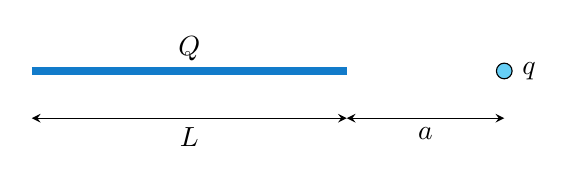
\begin{tikzpicture}[>=stealth]

    % Styles
    \tikzset{
        charge/.style={circle, draw=black, fill=cyan!60, inner sep=2pt},
        rod/.style={line width=3pt, cyan!60!blue, rounded corners=2pt}
    }

    % Coordinates
    \coordinate (A) at (0,0);         % left end of rod
    \coordinate (B) at (4,0);         % right end of rod  (represents length L)
    \coordinate (C) at (6,0);         % point charge position (distance a from B)

    % Rod
    \draw[rod] (A) -- (B);

    % Point charge
    \node[charge] (q) at (C) {};

    % Labels for the charges
    \node[above] at ($(A)!0.5!(B)$) {$Q$};
    \node[right] at (q.east) {$q$};

    % Distance L
    \draw[<->] (A) ++(0,-0.6) -- ++(4,0);
    \node[below] at ($(A)!0.5!(B) + (0,-0.6)$) {$L$};

    % Distance a
    \draw[<->] (B) ++(0,-0.6) -- ++(2,0);
    \node[below] at ($(B)!0.5!(C) + (0,-0.6)$) {$a$};

\end{tikzpicture}
\end{center}

In such a situation, we use \textit{charge density} to denote $Q / L$. Let $x$
be the distance from an arbitrary point in the segment and the charge $q$. Then

\begin{equation*}
    dQ = \frac{Q}{L} ~ dx
\end{equation*}

is the amount of charge in a segment of the line charge of length $dx$. Since we
can make $dx$ arbitrarily small, $dQ$ can be taken to represent a point charge,
so that we may use Coloumb's law.

\begin{center}
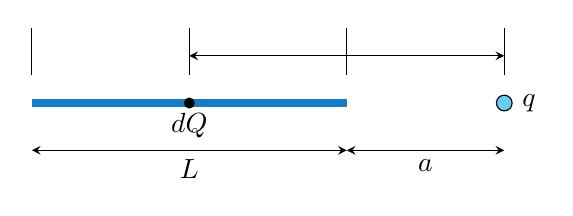
\begin{tikzpicture}[>=stealth]

    % Styles
    \tikzset{
        charge/.style={circle, draw=black, fill=cyan!60, inner sep=2pt},
        rod/.style={line width=3pt, cyan!60!blue, rounded corners=2pt},
        dq/.style={fill=black}
    }

    % Coordinates
    \coordinate (A) at (0,0);         % left end of rod
    \coordinate (B) at (4,0);         % right end of rod  (represents length L)
    \coordinate (C) at (6,0);         % point charge position (distance a)
    % Pick a point on the rod for the differential element dQ
    \coordinate (D) at (2,0);

    % Rod
    \draw[rod] (A) -- (B);

    % The differential charge element dQ
    \fill[dq] (D) circle (2pt);
    \node[below] at (D) {$dQ$};

    % Vertical markers (just like the textbook style)
    \draw (A) ++(0,0.35) -- ++(0,0.6);
    \draw (B) ++(0,0.35) -- ++(0,0.6);
    \draw (C) ++(0,0.35) -- ++(0,0.6);
    \draw (D) ++(0,0.35) -- ++(0,0.6);

    % Distance L
    \draw[<->] (A) ++(0,-0.6) -- ++(4,0);
    \node[below] at ($(A)!0.5!(B) + (0,-0.6)$) {$L$};

    % Distance a
    \draw[<->] (B) ++(0,-0.6) -- ++(2,0);
    \node[below] at ($(B)!0.5!(C) + (0,-0.6)$) {$a$};

    % Point charge q
    \node[charge] (q) at (C) {};
    \node[right] at (q.east) {$q$};

    % Distance x (from dq to the point charge q)
    \draw[<->] (D) ++(0,0.6) -- ++(4,0);


\end{tikzpicture}
\end{center}



\begin{equation*}
    d\vec{F} = \frac{1}{4\pi\epsilon_0} \frac{dQ \cdot q}{x^2} \hat{r}
\end{equation*}

Hence, since the force of multiple charges is additive, 

\begin{align*}
    \vec{F} = \int_{a}^{a+L} dF 
    &= \int_a^{a+L}  \frac{1}{4\pi\epsilon_0} \frac{dQ \cdot q}{x^2} \hat{r}\\ 
    & \frac{\hat{r}}{4\pi\epsilon_0} \int_{a}^{a+L} \frac{q \cdot Q /L }{x^2} ~ dx
\end{align*}

Note that $\hat{r}$ is constant: it always points either horizontally towards
$q$ or horizontally "against" $q$ (depending on whether $Q$ and $q$ are
identically charged or not). It is only for this reason that it can be factored
out of the integral. Now, solving the integral, we obtain

\begin{align*}
    \vec{F} = \frac{\hat{r}}{4\pi\epsilon_0} \int_{a}^{a+L} \frac{q \cdot Q /L }{x^2} ~ dx
    &= \frac{\hat{r} q \cdot Q}{L 4 \pi \epsilon_0} \int_{a}^{a+L} \frac{1}{x^2}
    ~ dx \\
    &= \hat{r} \cdot \frac{1}{4\pi \epsilon_0} \frac{qQ}{a(a+L)}
\end{align*}




\subsection{Electric fields}

Coloumb's law describes forces acting between two distant charges. However, we
can model the situation differently. Since any charged object $Q$ will exert
electrostatic force to other nearby charged objects, we can think of $Q$ as
creating a \textit{field} around it. Nearby objects are within this field at a
certain distance from $Q$, and the force in the field (due to Coloumb's law)
will be inversely proportional to the square of said distance.

Let $q$ by a charge nearby $Q$, or within the field of $Q$. Then

\begin{equation}\tag{Electric field}
    \vec{E} = \frac{\vec{F}}{q}
\end{equation}

Note that $\vec{E}$ is nothing but the \textit{normalized} force which $Q$
exerts to $q$. We can think of this as: the force which $Q$ would exert on an
object of charge $1+$. Note that the dimensions the electric field are newtons
over coulombs.

If we have multiple charges scattered in space, the electric field generated by
all of them is the sum of their individual fields: 

\begin{equation*}
    \vec{E} = \frac{1}{4\pi \epsilon 0}\sum_{i} \frac{q_i}{r^2} \hat{r_i}
\end{equation*}

Note that this is a vector sum. If the charges are smeared out in a continuous
distribution, the summation evolves into an integral:

\begin{equation*}
    \vec{E} = \frac{1}{4\pi \epsilon_0} \int \frac{dq}{r^2} \hat{r}
\end{equation*}

with $r$ the distance between each $dq$ and the location of interest. If said
distribution is uniform, and particularly linear, then the charge on each
segment is $\lambda = Q / L$ with $L$ the length of the segment in question. If
it is a surface, $\sigma = Q / A$ with $A$ the area is the charge on each point.
If it is a 3D distribution, $\varrho = Q / V$ is the charge per volume. So: 

\begin{itemize}
    \item For linear distributions of charge, $dq = \lambda ~ \text{dl}$
    \item For surface distributions, $dq = \sigma \text{ ds}$
    \item For volumetric distributions, $dq = \varrho \text{ dv}$
\end{itemize}

where dl, ds and dv are the infinitesimal regions of a line, a surface or a
volume, respectively.


\begin{center}
\begin{tikzpicture}[scale=1]
  % Styles
  \tikzset{
    charge/.style={circle,draw=black,fill=white,inner sep=1.5pt,font=\bfseries},
    fieldline/.style={->,>=Stealth,thick},
    equip/.style={dashed,gray}
  }

  % Positive point charge at origin
  \node[charge] (q) at (0,0) {+};

  % Radial field lines (arrows pointing outward)
  \foreach \a in {0,30,...,330}{
    \draw[fieldline] ($(0,0)!0.18!(\a:2.5)$) -- (\a:2.5);
  }

  % A few long field lines to show they go to infinity
  \foreach \a in {15,75,135,195,255,315}{
    \draw[fieldline] ($(0,0)!0.18!(\a:4.0)$) -- (\a:4.0);
  }

  % Equipotential circles
  \foreach \r in {0.8,1.6,2.4,3.2}{
    \draw[equip] (0,0) circle (\r);
  }

  % Labels
  \node[align=center, right] at (4.4,0) {Electric field lines\\point outward from $+q$};
  \node[gray!60] at (0,3.6) {Equipotentials (dashed)};
\end{tikzpicture}
\end{center}

\begin{center}
\begin{tikzpicture}[scale=1]
  % Styles
  \tikzset{
    charge/.style={circle,draw=black,fill=white,inner sep=1.5pt,font=\bfseries},
    fieldline/.style={->,>=Stealth,thick},
    faint/.style={gray,font=\footnotesize}
  }

  % Charges positions
  \coordinate (P) at (-1.2,0); % positive
  \coordinate (N) at (1.2,0);  % negative

  % Draw charges
  \node[charge] at (P) {+};
  \node[charge] at (N) {--};

  % Field lines that start near + and end at - (a few representative ones)
  % We'll draw symmetric sets above and below the axis.
  \foreach \t/\outA/\inB in {
    0/15/165, 1/30/150, 2/45/135, 3/75/105,
    4/-15/-165, 5/-30/-150, 6/-45/-135, 7/-75/-105
  }{
    % start point near positive charge on a small circle
    \pgfmathsetmacro{\angleA}{\outA}
    \pgfmathsetmacro{\angleB}{\inB}
    \draw[fieldline] ($(P)+(\angleA:0.28)$) to[out=\angleA,in=\angleB] ($(N)+(\angleB:0.28)$);
  }

  % Some lines that emanate outward from positive and go to infinity
  \foreach \a in {10,350,80,280}{
    \draw[fieldline] ($(P)+(\a:0.28)$) -- ($(P)+(\a:4.0)$);
  }
  % Some lines that come from infinity into negative
  \foreach \a in {170,190,100,260}{
    \draw[fieldline] ($(N)+(\a:4.0)$) -- ($(N)+(\a:0.28)$);
  }

  % Axis and labels
  \draw[dashed,gray] (-3.5,0) -- (3.5,0);
  \node[faint] at (0,-0.6) {Dipole axis};
  \node[below left] at (P) {$+q$};
  \node[below right] at (N) {$-q$};

  % Field direction explanation
  \node[align=left] at (4.3,1.4) {
    Field lines start on $+$ and end on $-$;\\
    lines between charges show attraction.
  };
\end{tikzpicture}
\end{center}


\subsection{Electric potential and electric potential energy}

Electric potential energy is the negative of the work needed to move a charge
\textit{against} an electric field and into some reference position. 
Electric potential depends on the distance of the movement, the magnitude of the
charge, and the strengt of the electric field: 

\begin{itemize}
    \item Weak electric field, long distance $\to $ medium electric potential 
    \item Strong electric field, long distance $\to$ High electric potential 
    \item Weak electric field, short distance $\to $ Low electric potential
    \item Weak electric field, high distance $\to $ Medium electric potential
\end{itemize}

(Of course the items above are only schematic.) 

Electric potential, also called \textbf{voltage}, is the \textit{difference} in
potential energy per unite charge between two locations in an electric field.
Why per unit charge? Well, we have already established that 













































\end{document}


